\section{Tables}
\begin{table}[H]
    \centering
    \caption{Summary Statistics}
    \label{tab:descriptive-statistic}
{\small

\begin{tabular}{lrr}
\toprule
{} &      mean &          std \\
\midrule
host\_is\_superhost      &     0.234 &        0.424 \\
host\_listings\_count    &     7.775 &       54.391 \\
host\_identity\_verified &     0.486 &        0.500 \\
accommodates           &     2.906 &        1.911 \\
bathrooms              &     1.140 &        0.421 \\
bedrooms               &     1.183 &        0.750 \\
beds                   &     1.570 &        1.156 \\
price                  &   138.085 &      118.185 \\
security\_deposit       &   172.822 &      406.817 \\
cleaning\_fee           &    54.161 &       54.671 \\
guests\_included        &     1.584 &        1.210 \\
extra\_people           &    15.986 &       25.143 \\
minimum\_nights         &     6.151 &       19.285 \\
maximum\_nights         & 55397.541 & 10750846.675 \\
availability\_90        &    32.857 &       33.807 \\
number\_of\_reviews      &    31.090 &       51.014 \\
instant\_bookable       &     0.382 &        0.486 \\
host\_days\_active       &  1654.499 &      885.855 \\
air\_conditioning       &     0.867 &        0.339 \\
bed\_linen              &     0.349 &        0.477 \\
tv                     &     0.685 &        0.465 \\
coffee\_machine         &     0.339 &        0.473 \\
cooking\_basics         &     0.370 &        0.483 \\
white\_goods            &     0.447 &        0.497 \\
elevator               &     0.250 &        0.433 \\
child\_friendly         &     0.280 &        0.449 \\
parking                &     0.469 &        0.499 \\
host\_greeting          &     0.171 &        0.377 \\
internet               &     0.984 &        0.126 \\
long\_term\_stays        &     0.218 &        0.413 \\
pets\_allowed           &     0.165 &        0.371 \\
private\_entrance       &     0.210 &        0.407 \\
self\_check\_in          &     0.260 &        0.438 \\
\bottomrule
\end{tabular}
}
\end{table}

\begin{flushleft}
\begin{table}[H]
    \caption{The variable list}
    \label{tab:variable-list}
    {\small
    \begin{tabular}{ll}
    \hline
    Variables & Definition \\
    \hline
    experience\_offerd & recommended category of travel type, e.g. business \\
    host\_since & date that the host first joined Airbnb \\
    host\_response\_time & average amount of time the host takes to reply to messages \\
    host\_response\_rate & proportion of messages that the host replies to \\
    host\_is\_superhost &
    \begin{tabular}{@{}l@{}l@{}} whether or not the host is a superhost, which is a
        mark of \\ mark of quality for the top-rated and most experienced hosts,
        \\ and can increase your search ranking on Airbnb \end{tabular} \\
    host\_listings\_count & how many listings the host has in total \\
    host\_identity\_verified & whether or not the host has been verified with id \\
    neighbourhood\_cleansed & NewYork  borough the property is in \\
    property\_type & type of property, e.g. house or flat \\
    room\_type & type of listing, e.g. entire home, private room or shared room \\
    accommodates & how many people the property accommodates \\
    bathrooms & number of bathrooms \\
    bedrooms & number of bedrooms \\
    beds & number of beds \\
    bed\_type & type of bed, e.g. real bed or sofa-bed \\
    amenities & list of amenities \\
    price & nightly advertised price (the target variable) \\
    security\_deposit & the amount required as a security deposit \\
    cleaning\_fee & the amount of the cleaning fee (a fixed amount paid per booking)
    \\
    guests\_included & the number of guests included in the booking fee \\
    extra\_people & the price per additional guest above the guests\_included price
    \\
    minimum\_nights & the minimum length of stay \\
    maximum\_nights & the maximum length of stay \\
    calendar\_updated & when the host last updated the calendar \\
    availability\_30 & how many nights are available to be booked in the next 30
    days \\
    availability\_60 & how many nights are available to be booked in the next 60
    days \\
    availability\_90 & how many nights are available to be booked in the next 90
    days \\
    availability\_365 & how many nights are available to be booked in the next
    365 days \\
    number\_of\_reviews & the number of reviews left for the property \\
    number\_of\_reviews\_ltm & the number of reviews left for the property in the
    last twelve months \\
    first\_review & the date of the first review \\
    last\_review & the date of the most recent review \\
    review\_scores\_rating & guests can score properties overall from 1 to 5 stars
    \\
    review\_scores\_accuracy &  accuracy score of a property's description from 1 to 5 stars \\
    review\_scores\_cleanliness & guests can score a property's cleanliness from 1
    to 5 stars \\
    review\_scores\_checkin & guests can score their check-in from 1 to 5 stars \\
    review\_scores\_communication & guests can score a host's communication from 1
    to 5 stars \\
    review\_scores\_location & guests can score a property's location from 1 to 5
    stars \\
    review\_scores\_value & guests can score a booking's value for money from 1 to 5
    stars \\
    instant\_bookable &
    \begin{tabular}{@{}l@{}l@{}}
            whether or not the property can be instant booked (i.e.
            booked \\ straight away, without having to message the host first
            and wait to \\ be accepted)
        \end{tabular} \\
    cancellation\_policy & the type of cancellation policy, e.g. strict or moderate \\
    reviews\_per\_month & average number of reviews left by guest each month \\
\end{tabular}
}
\end{table}
\end{flushleft}


\section{Figures}

\begin{figure}[H] \centering
    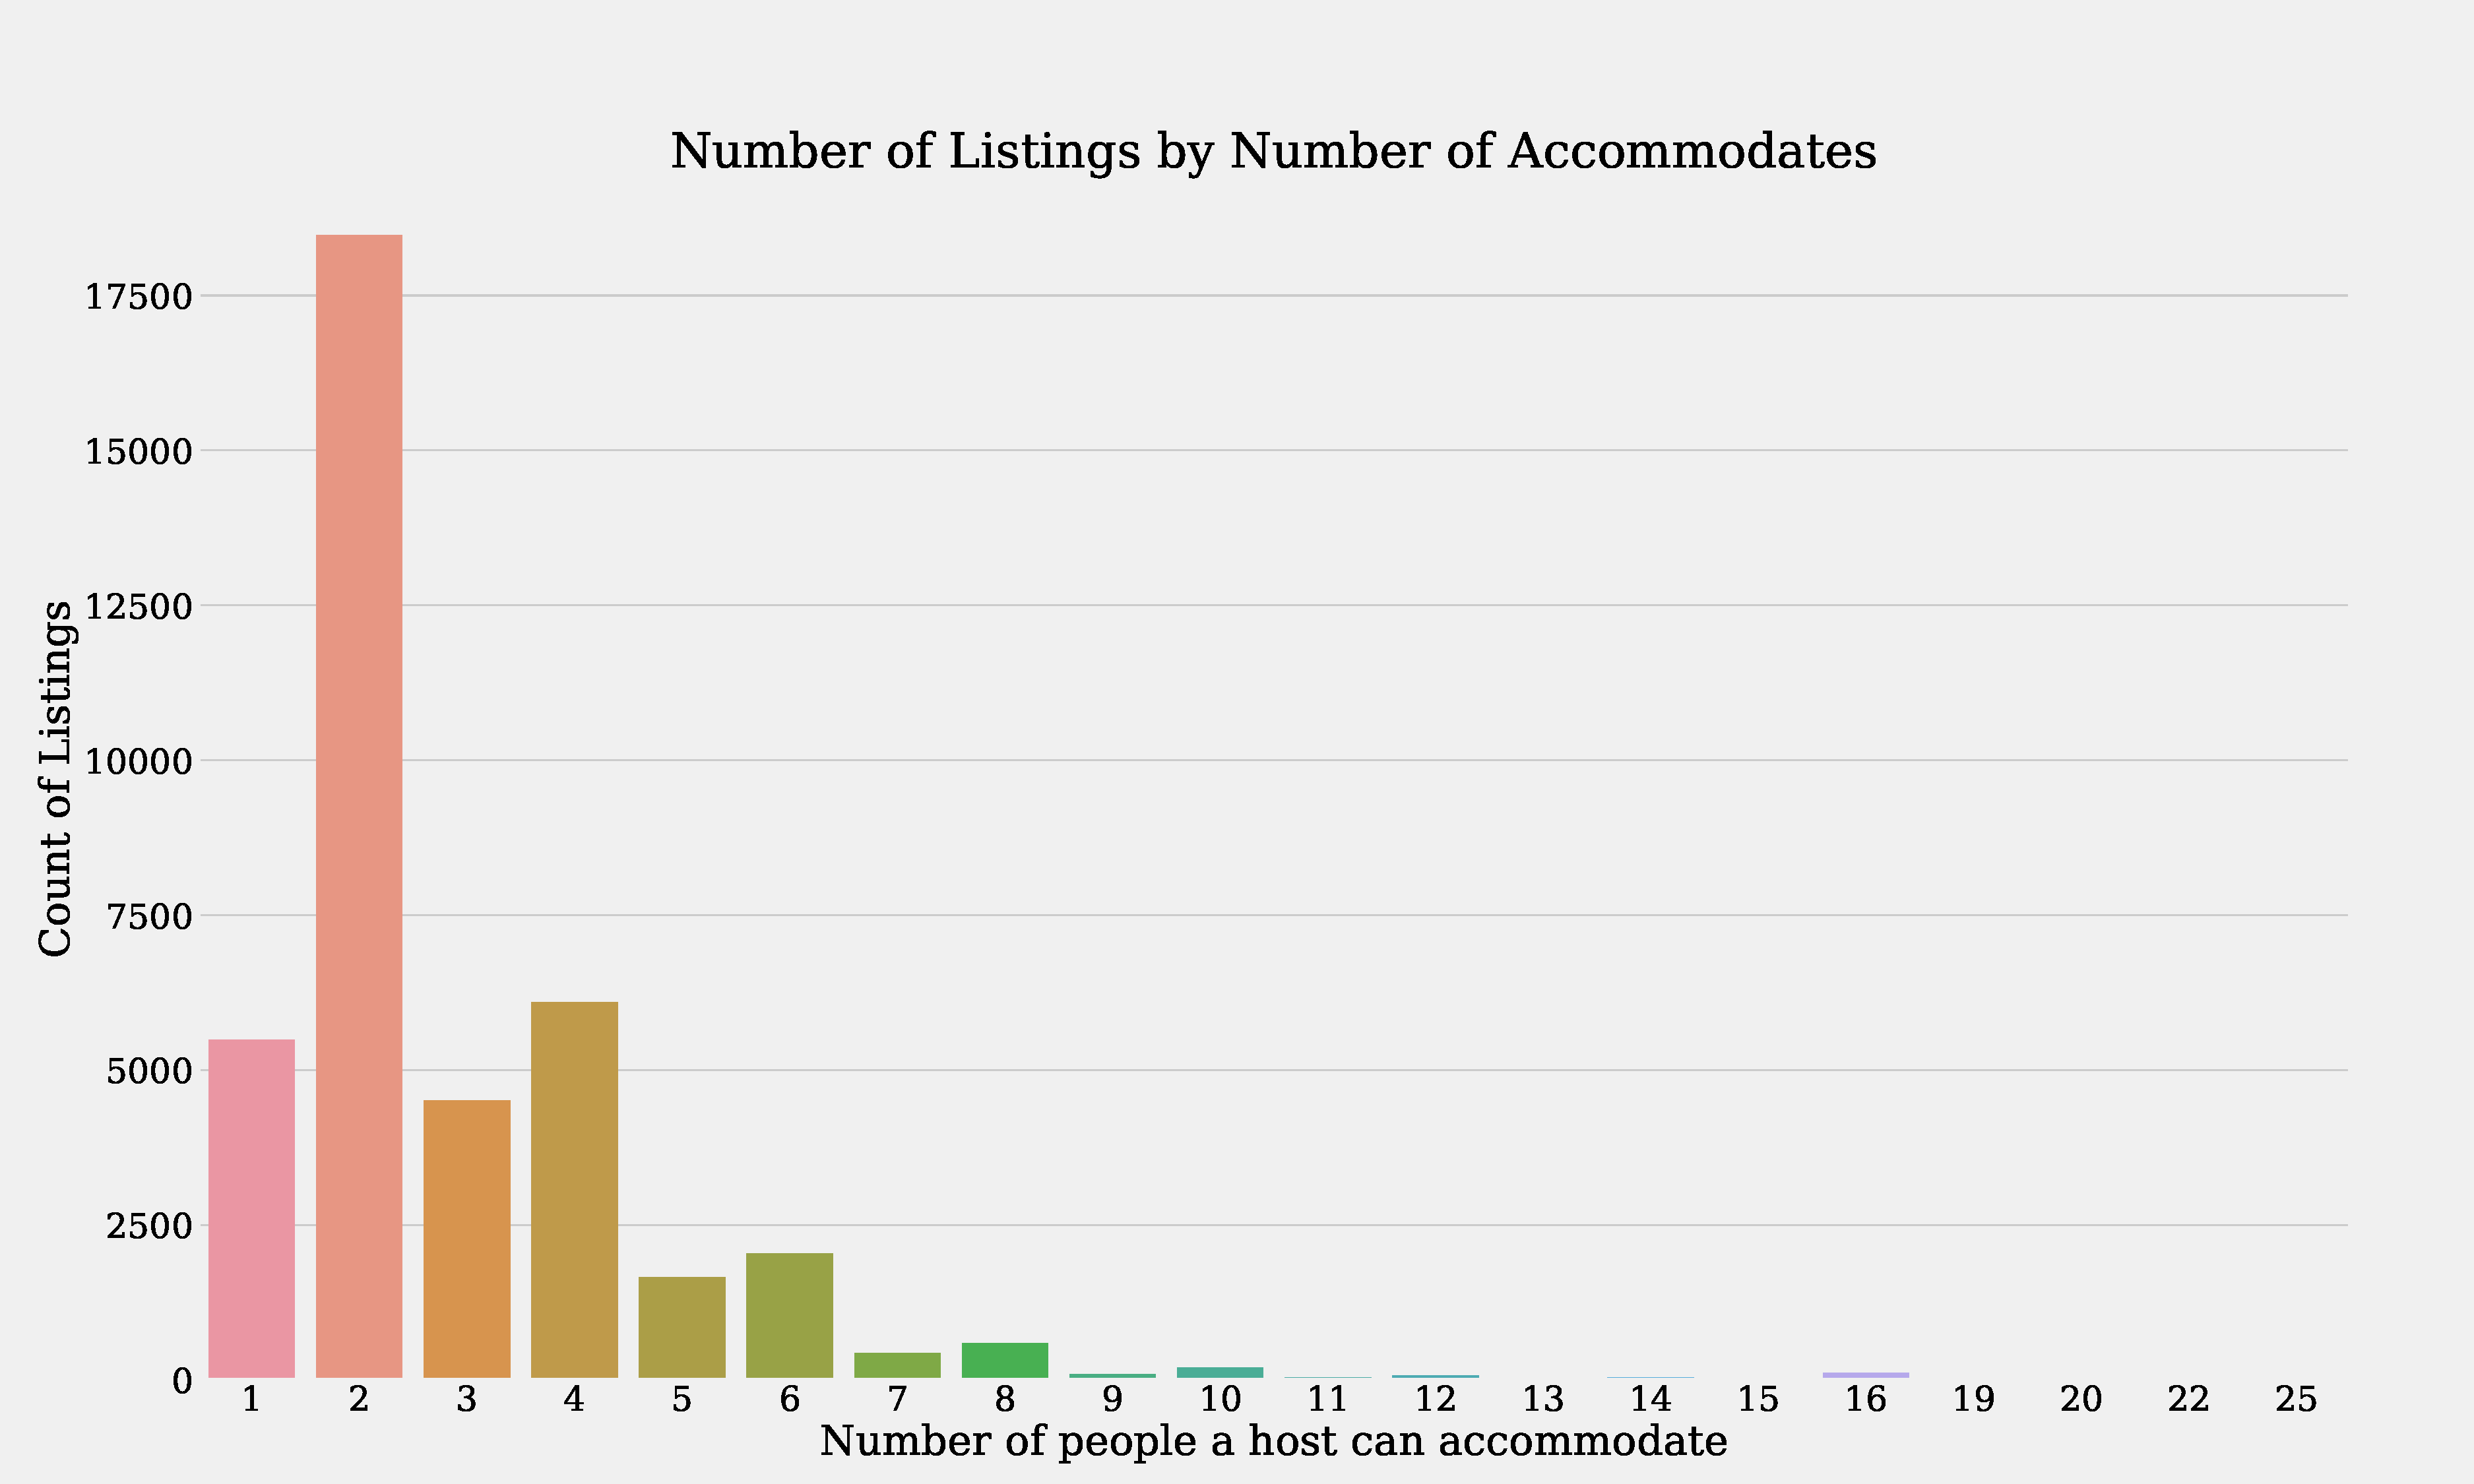
\includegraphics[width=\textwidth]{accommodates-countplot.pdf}
    \caption{Number of Listings by Accomodates}
    \label{fig:accommodates-countplot}
\end{figure}

\begin{figure}[H] \centering
    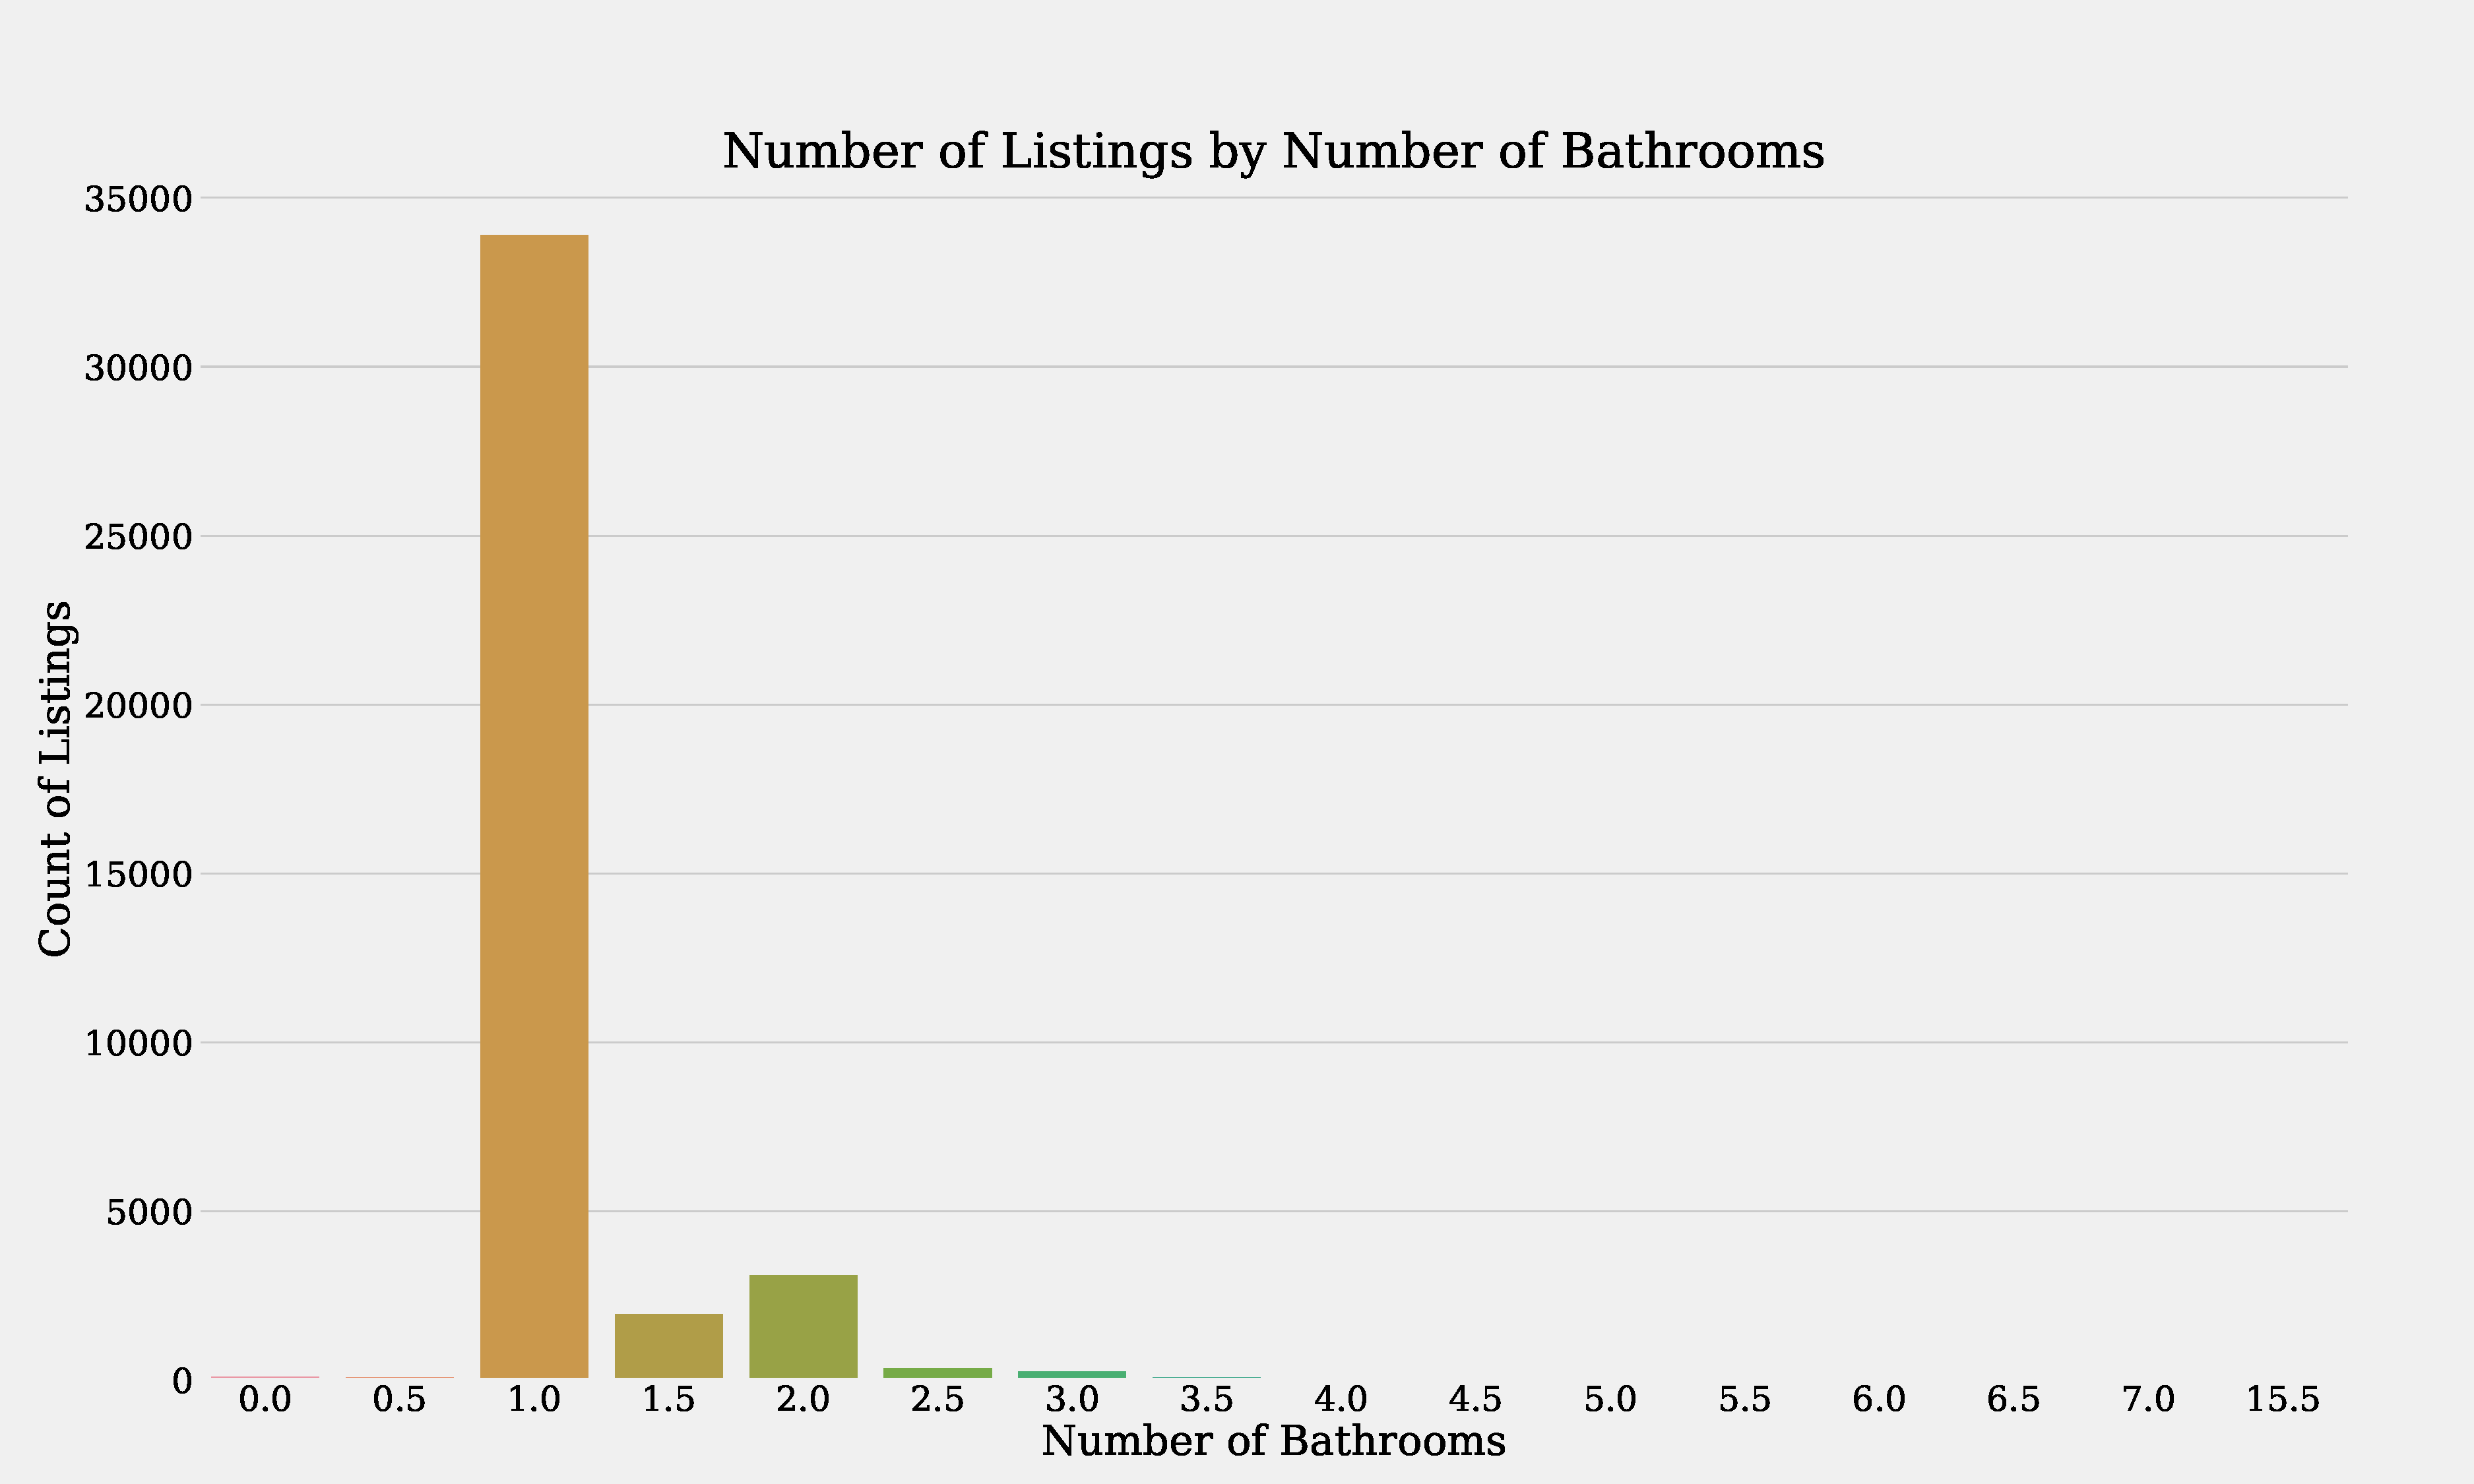
\includegraphics[width=\textwidth]{bathrooms-countplot.pdf}
    \caption{Number of Listings by Number of Bathrooms }
    \label{fig:bathrooms-countplot}
\end{figure}

\begin{figure}[H] \centering
    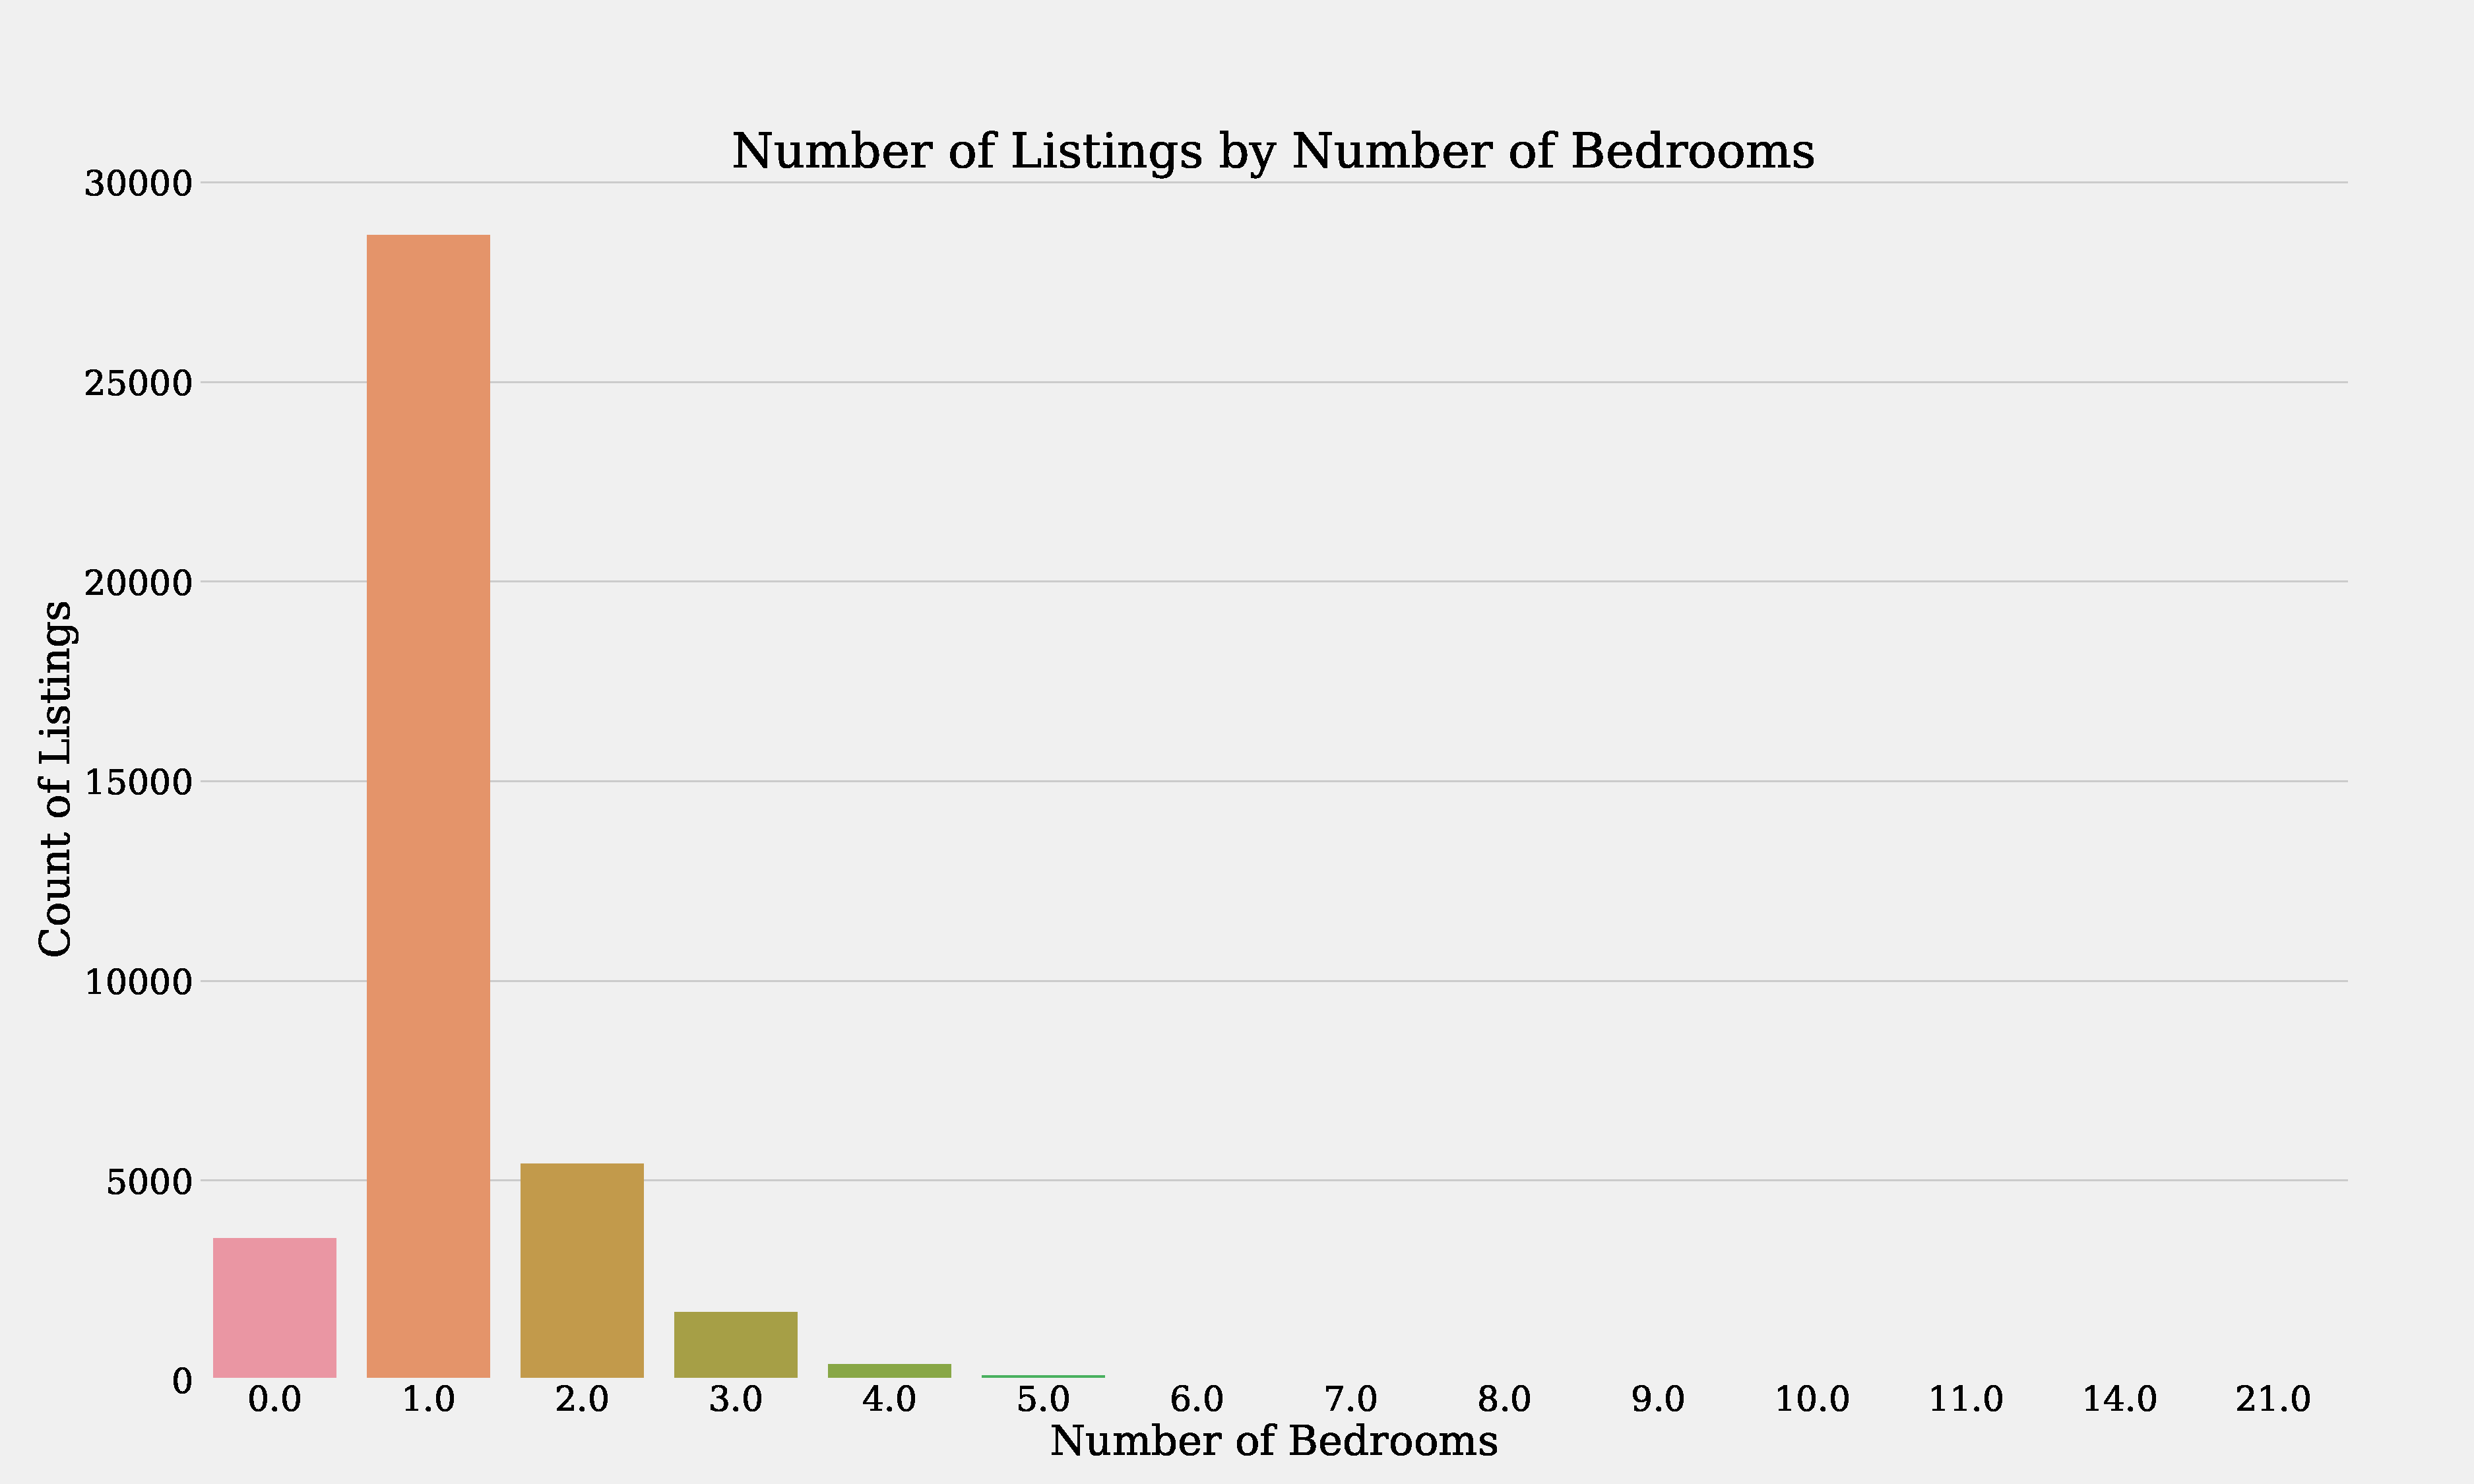
\includegraphics[width=\textwidth]{bedrooms-countplot.pdf}
    \caption{Number of Listings by Number of Bedrooms }
    \label{fig:bedrooms-countplot}
\end{figure}

\begin{figure}[H] \centering
    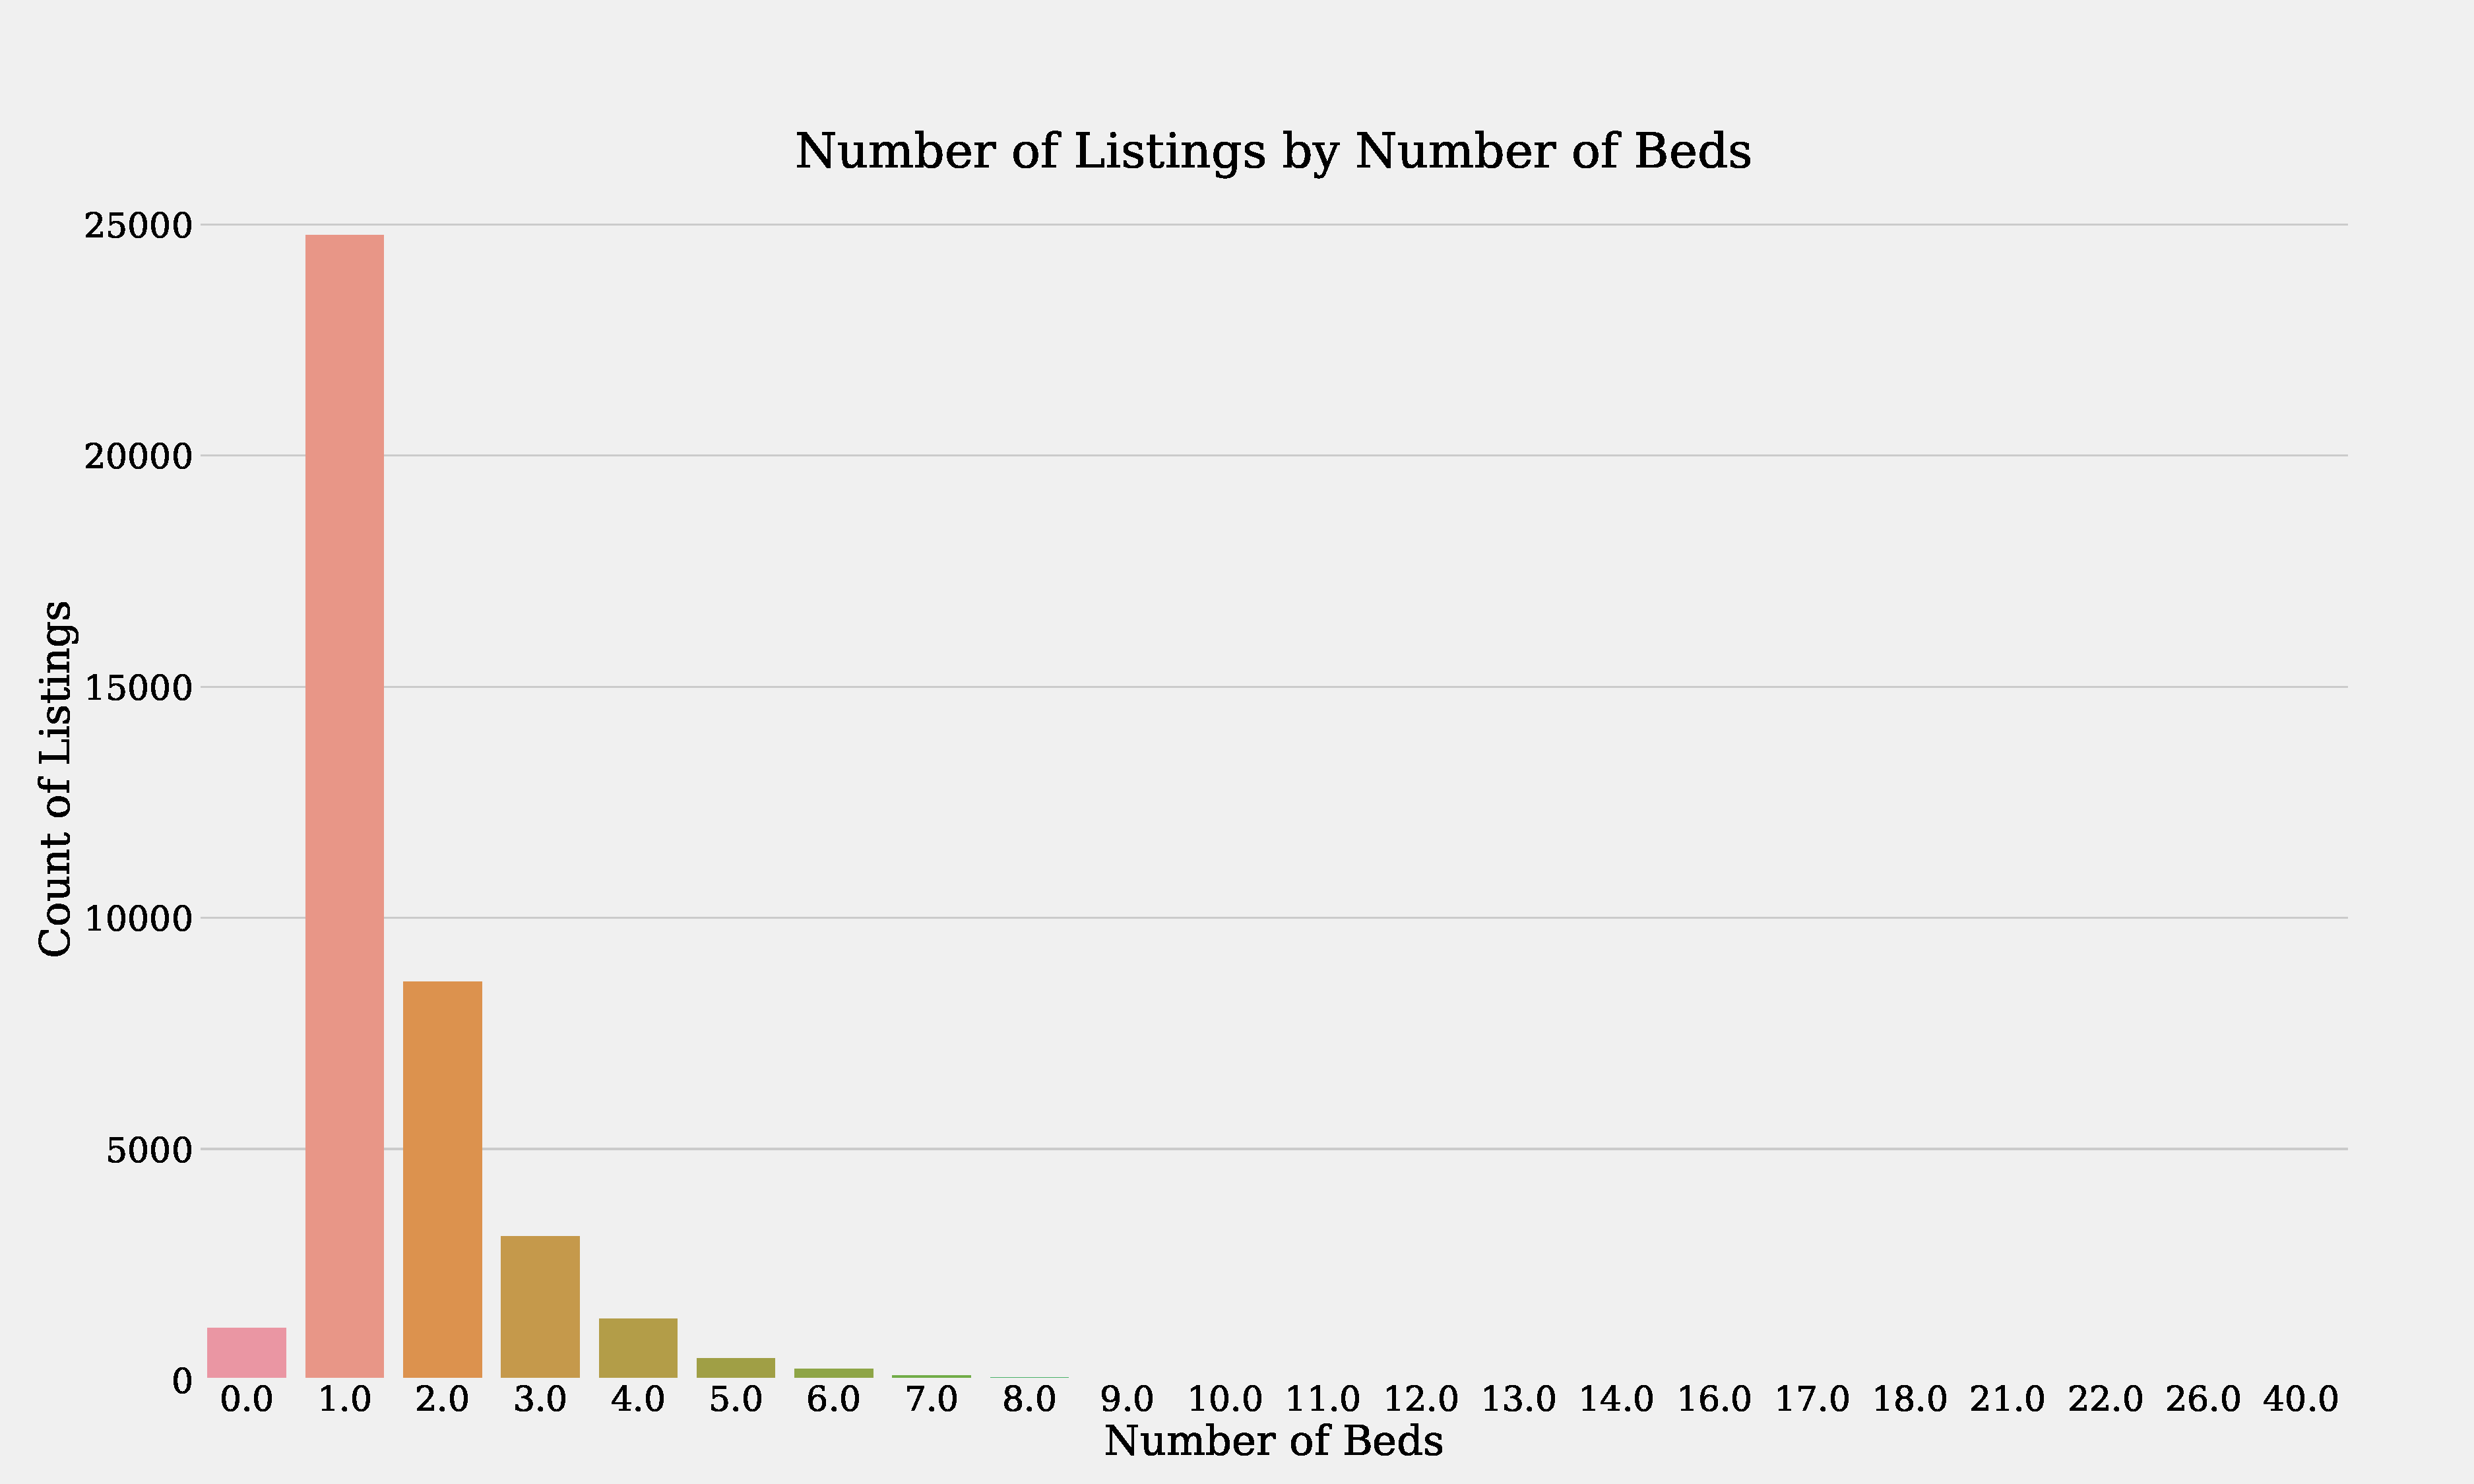
\includegraphics[width=\textwidth]{beds-countplot.pdf}
    \caption{Number of Listings by Number of Beds }
    \label{fig:beds-countplot}
\end{figure}

% ------------------------------
% median price by accommodates, bathrooms, bedrooms, beds
\begin{figure}[H] \centering
    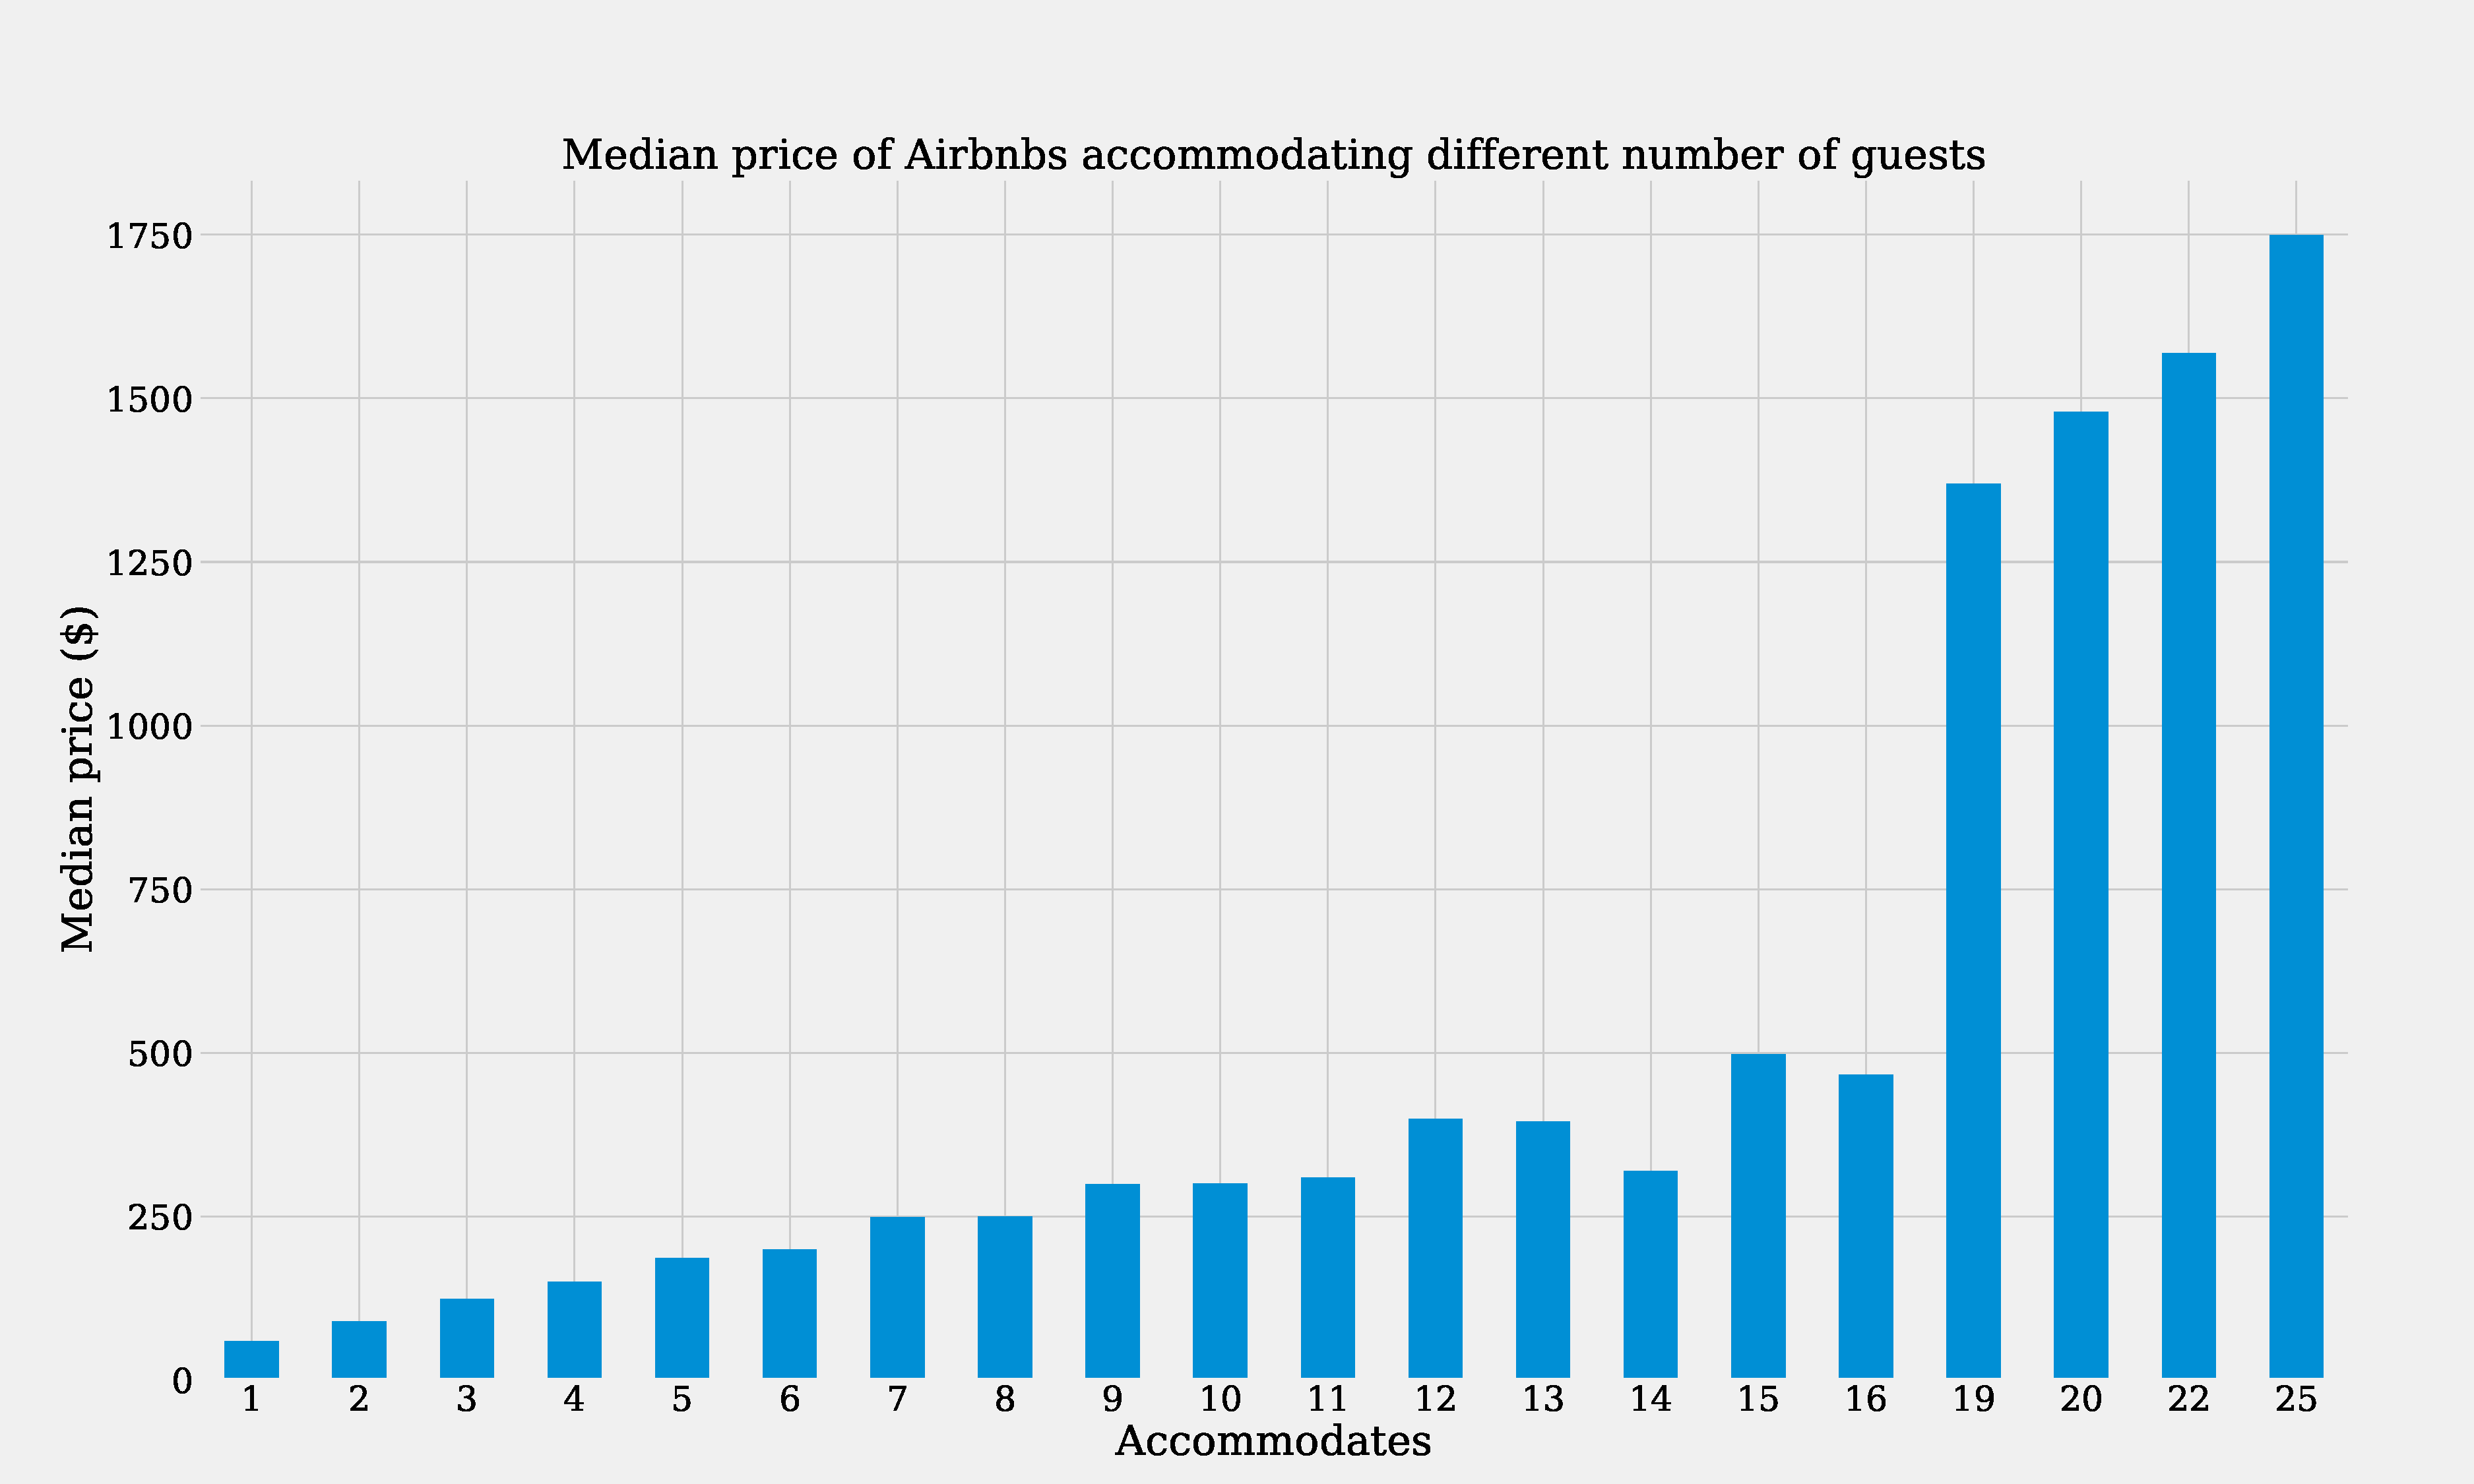
\includegraphics[width=\textwidth]{median-price-by-accommodates.pdf}
    \caption{Median Price By Accommodates}
    \label{fig:median-price-by-accommodates}
\end{figure}

\begin{figure}[H] \centering
    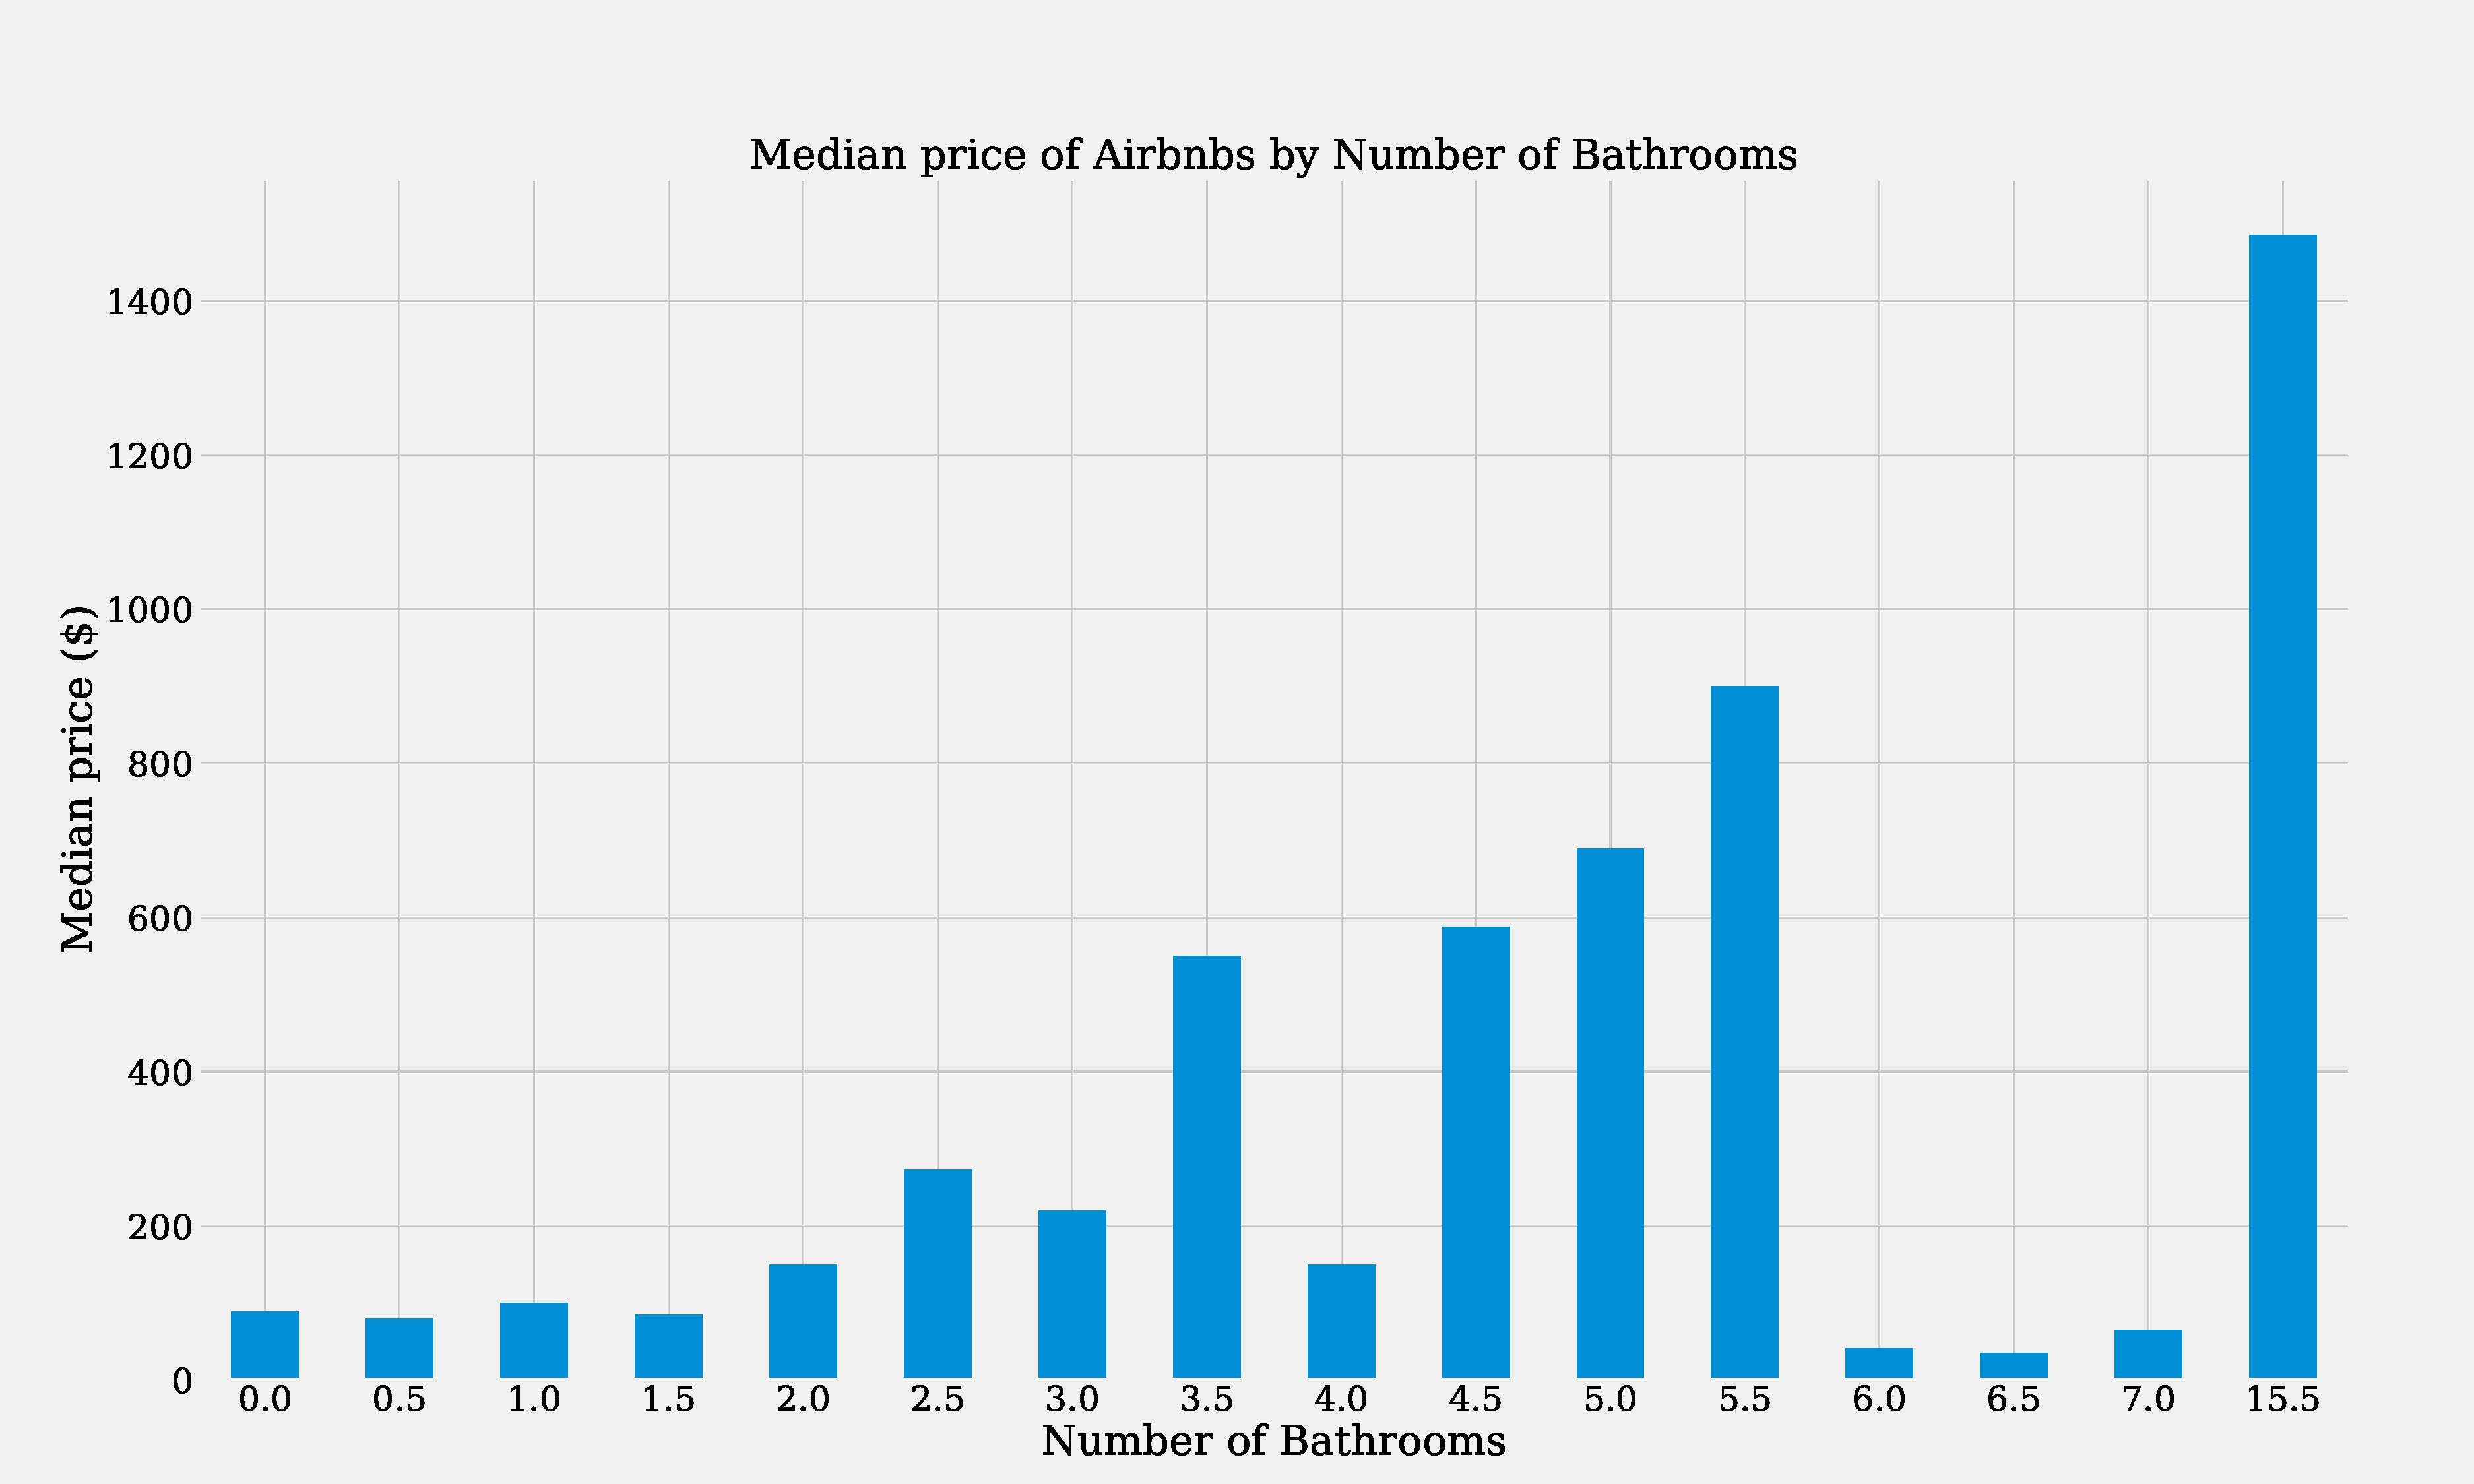
\includegraphics[width=\textwidth]{median-price-by-bathrooms.pdf}
    \caption{Median Price By  Number of Bathrooms }
    \label{fig:median-price-by-bathrooms}
\end{figure}

\begin{figure}[H] \centering
    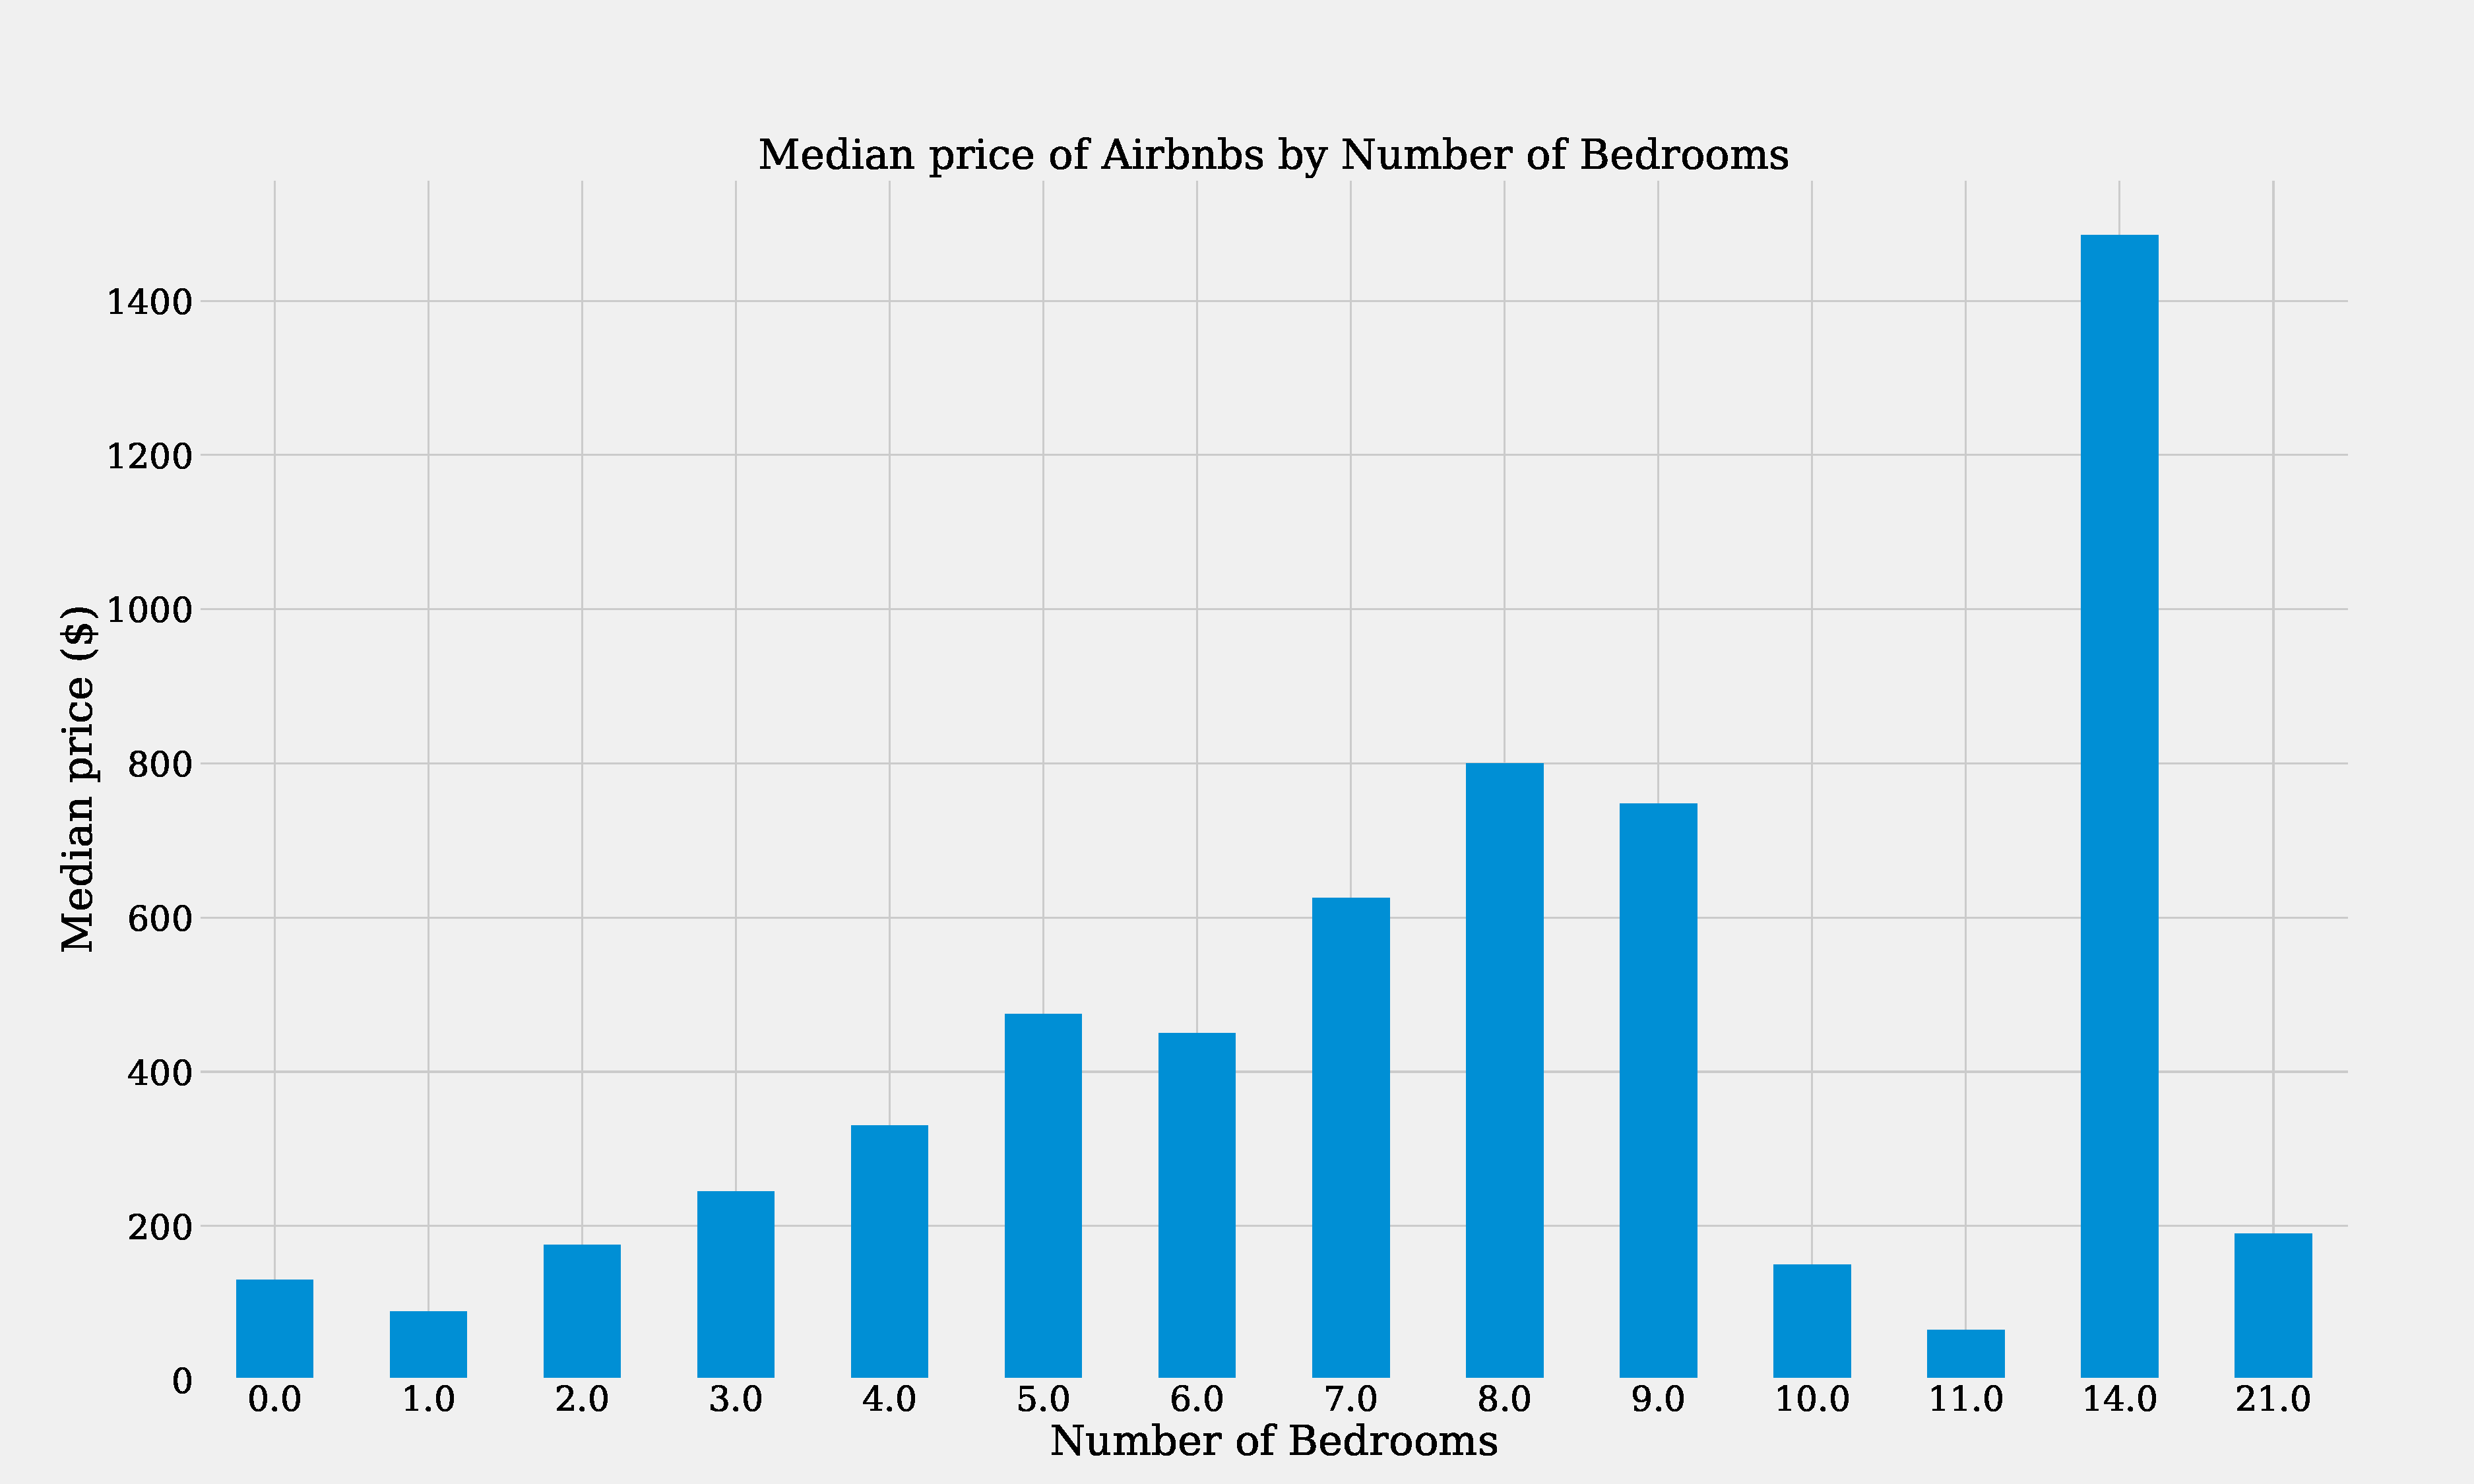
\includegraphics[width=\textwidth]{median-price-by-bedrooms.pdf}
    \caption{Median Price By Number of Bedrooms}
    \label{fig:median-price-by-bedrooms}
\end{figure}


\begin{figure}[H] \centering
    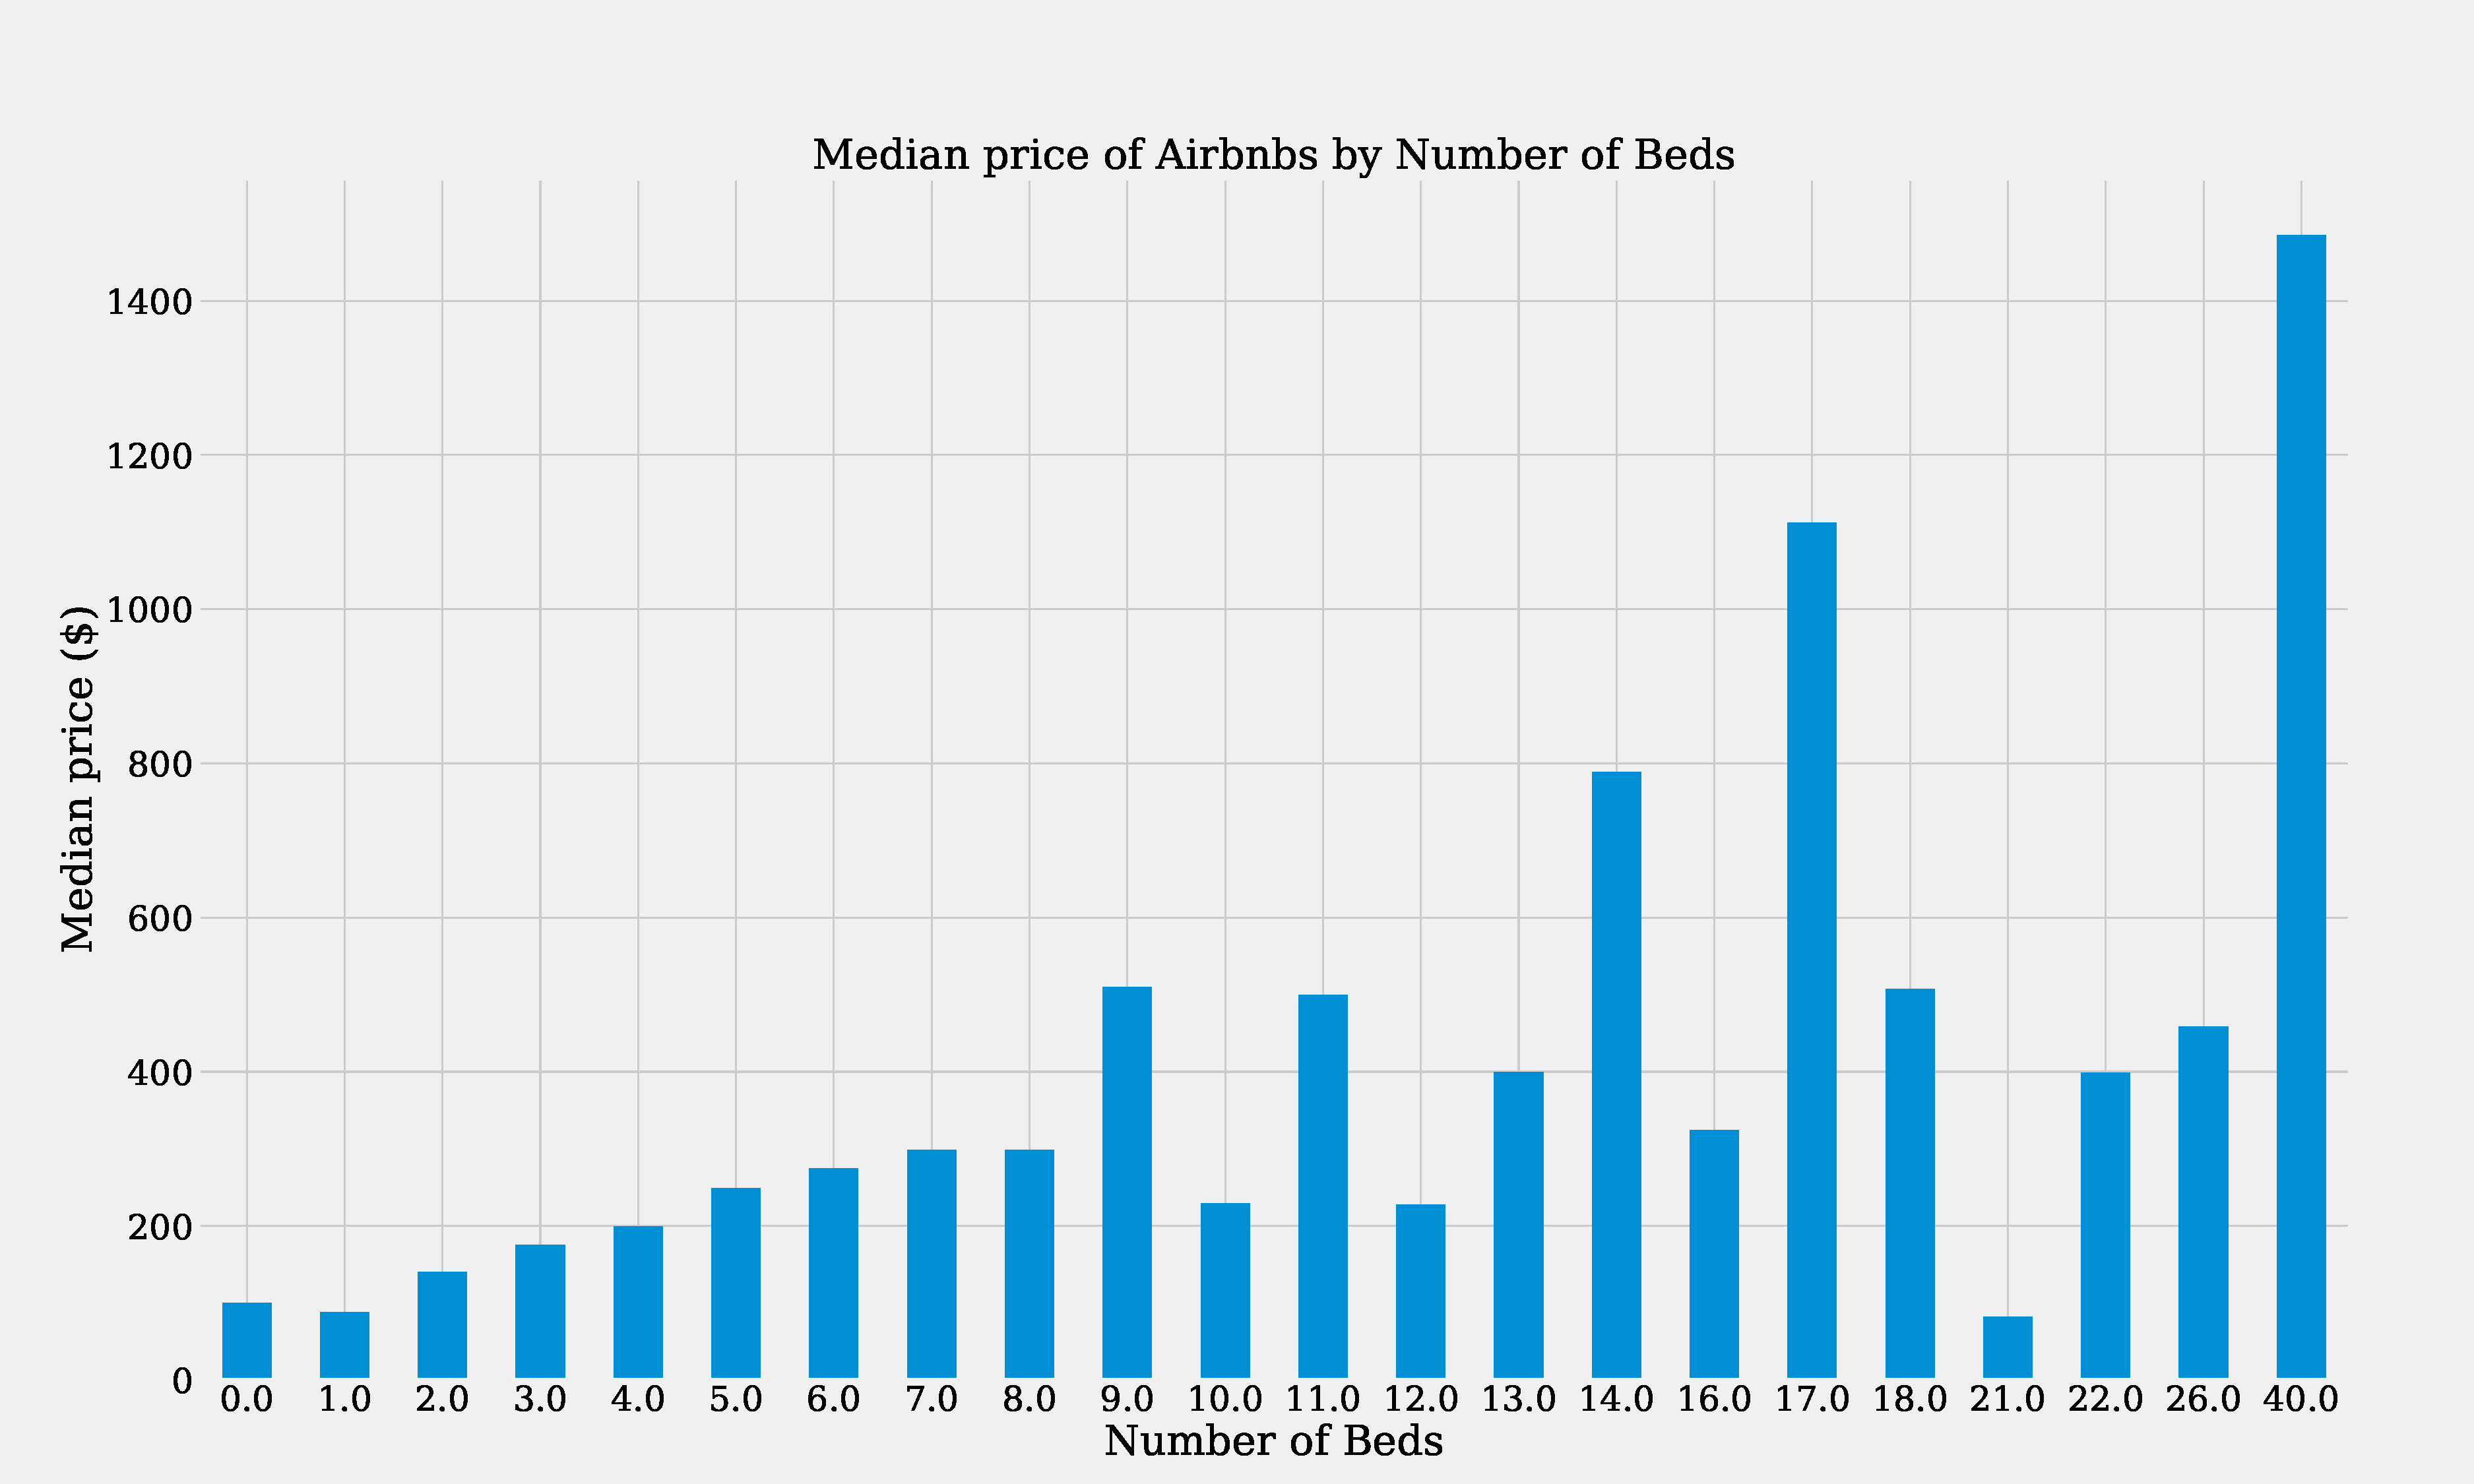
\includegraphics[width=\textwidth]{median-price-by-beds.pdf}
    \caption{Median Price By Number of Beds}
    \label{fig:median-price-by-beds}
\end{figure}

% ------------------------------

% Amenity Group 1
\begin{figure}[H]
\centering
    \caption{Elevator and Bed Linen}
    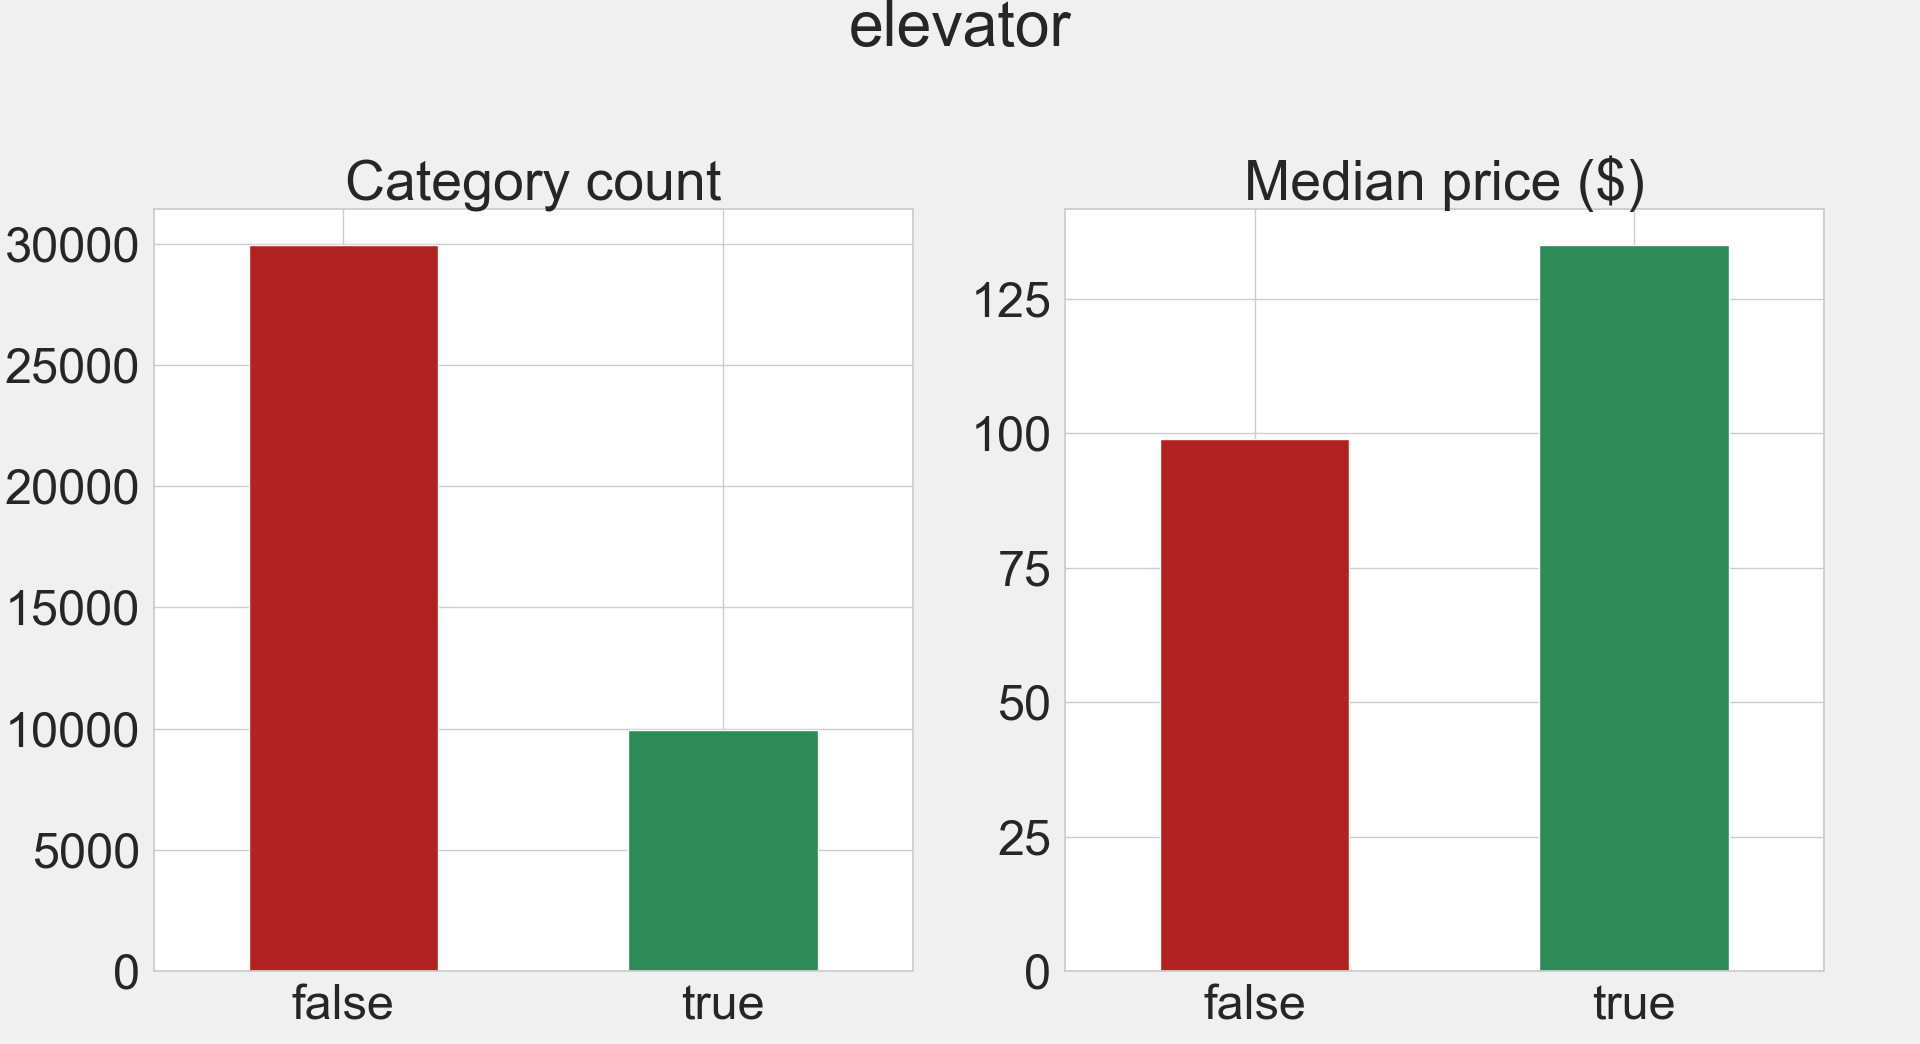
\includegraphics[width=\linewidth]{figures/amenities/group1/elevator.png}
    %\caption{Caption 1}
    \vspace{0.3cm}
    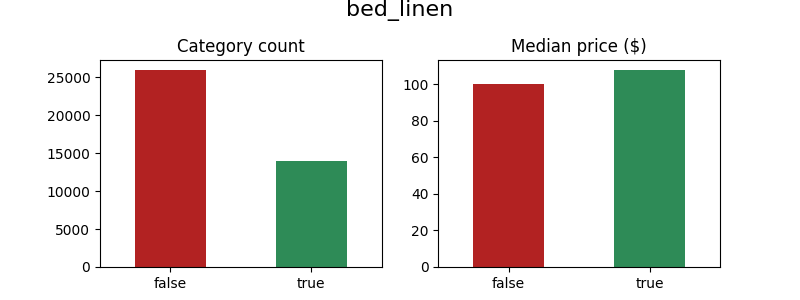
\includegraphics[width=\linewidth]{figures/amenities/group1/bed_linen.png}
    %\caption{Caption 2}
    \label{fig:elevator-and-bed-linen}
\end{figure}


\begin{figure}[H]
\centering
\caption{White Goods and Pets Allowed}
    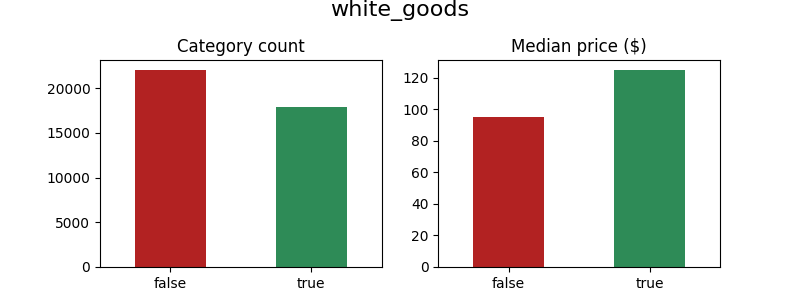
\includegraphics[width=\linewidth]{figures/amenities/group1/white_goods.png}
    %\caption{Caption 1}
    \vspace{0.5cm}
    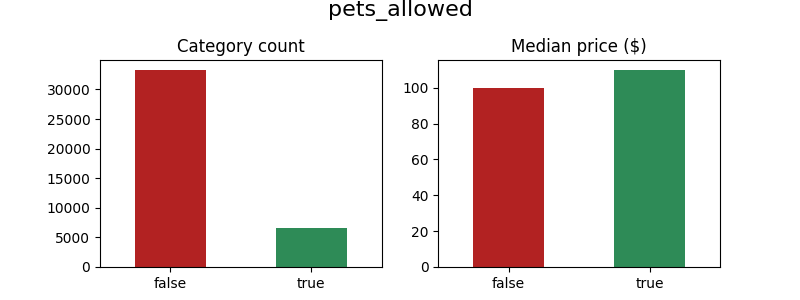
\includegraphics[width=\linewidth]{figures/amenities/group1/pets_allowed.png}
    %\caption{Caption 2}
    \label{fig:white-goods-and-pets-allowed}
    \
\end{figure}

\begin{figure}[H]
\centering
\caption{Self Check In and Coffee Machine}
    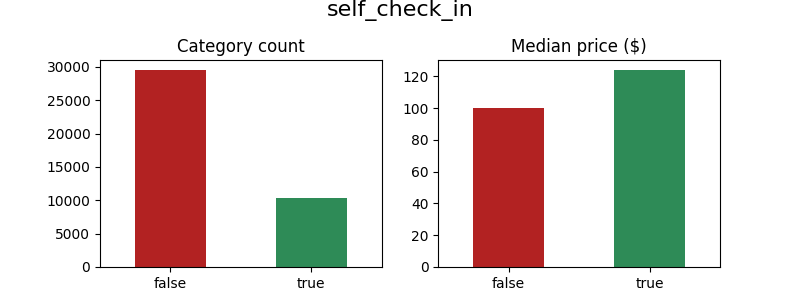
\includegraphics[width=\linewidth]{figures/amenities/group1/self_checkin.png}
    %\caption{Caption 1}
    \vspace{0.5cm}
    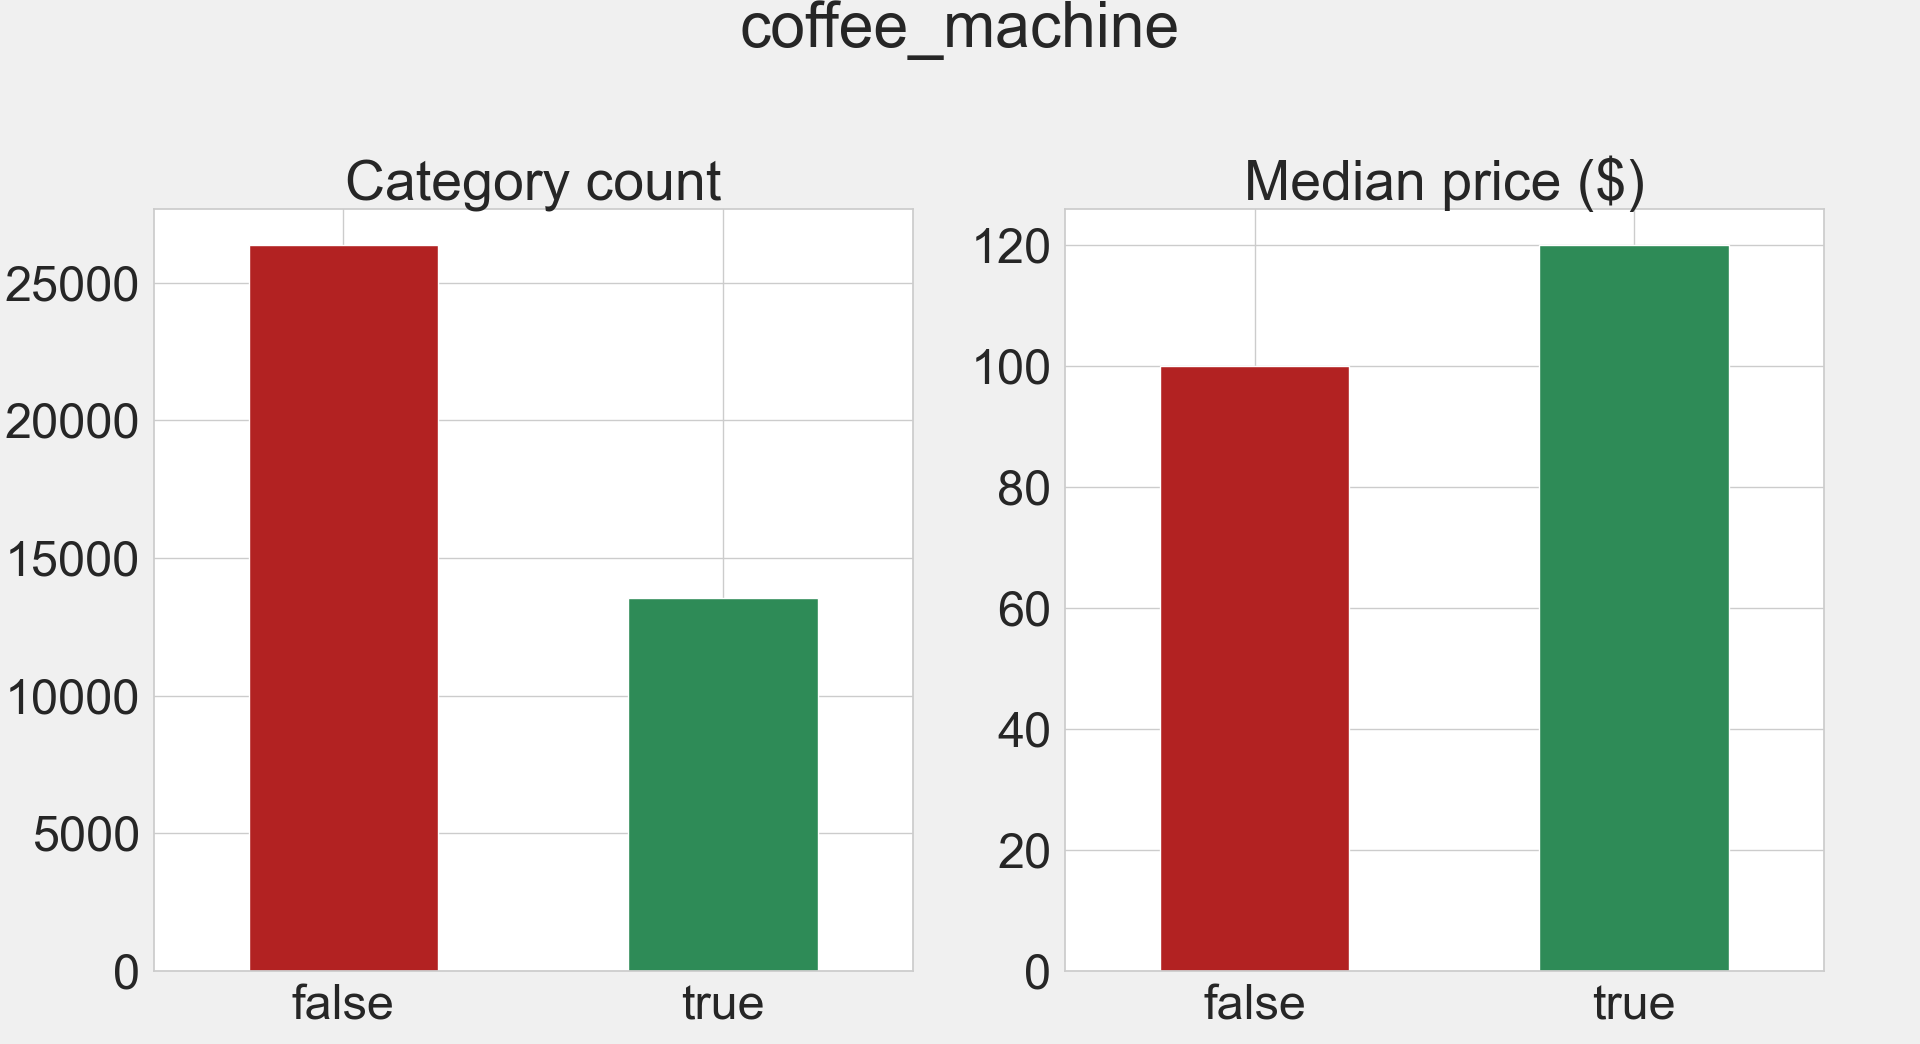
\includegraphics[width=\linewidth]{figures/amenities/group1/coffee_machine.png}
    %\caption{Caption 2}
    \label{fig:self-checkin-and-coffee-machine}
\end{figure}

\begin{figure}[H]
    \centering
    \caption{Long Term Stays and Child Friendly}
    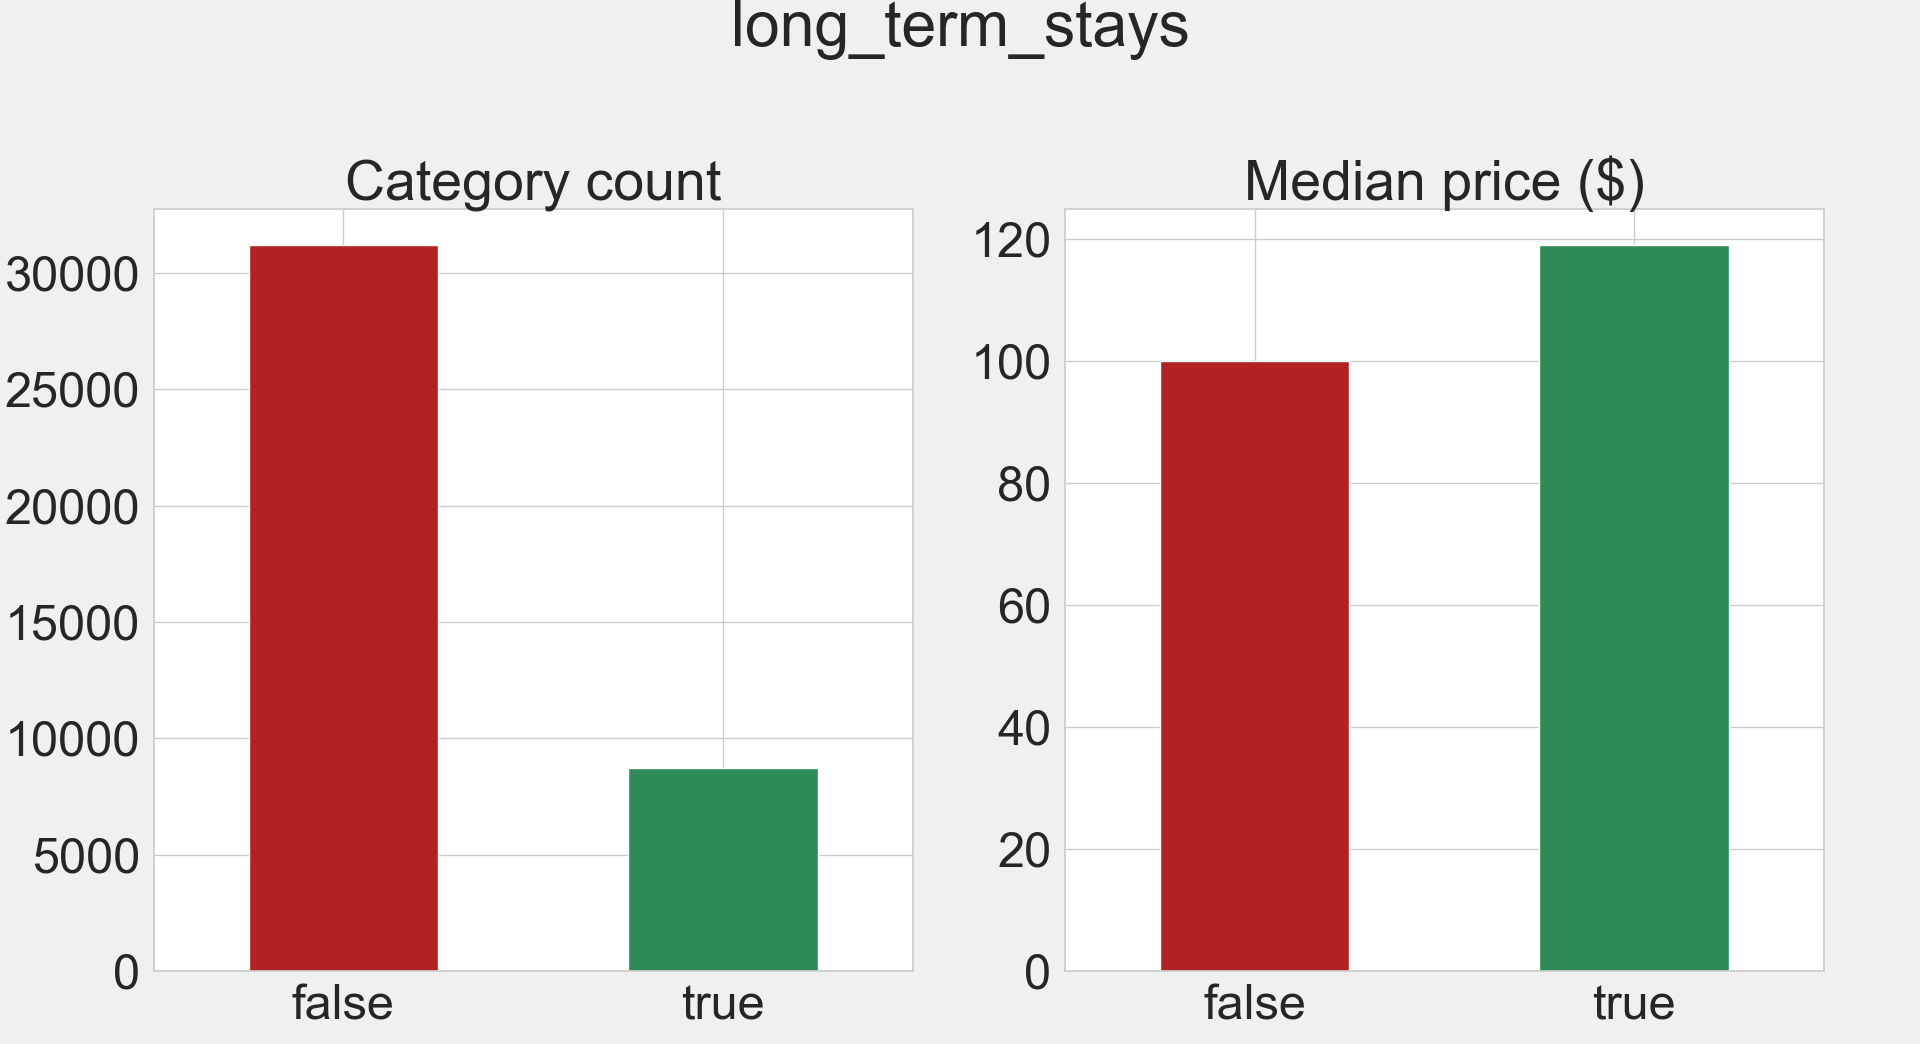
\includegraphics[width=\linewidth]{figures/amenities/group1/long_term_stays.png}
    %\caption{Caption 1}
    \vspace{0.5cm}
    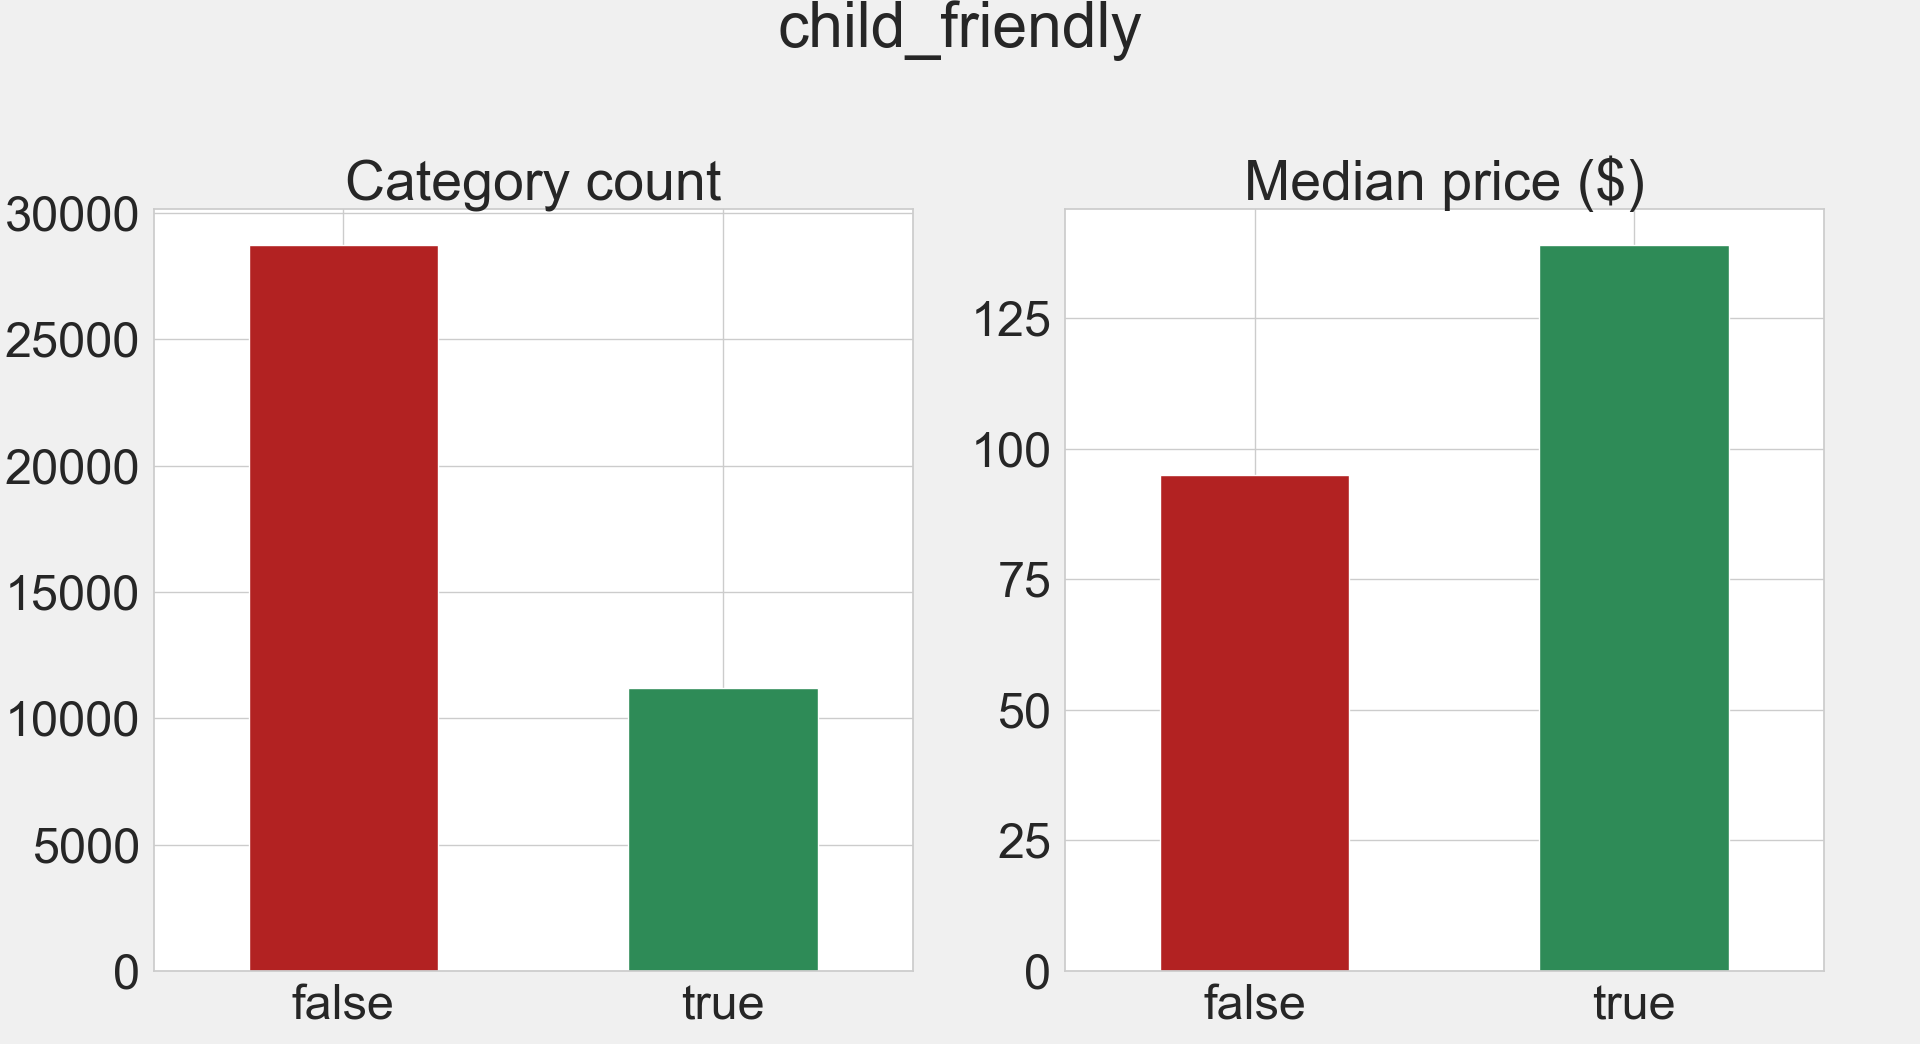
\includegraphics[width=\linewidth]{figures/amenities/group1/child_friendly.png}
    %\caption{Caption 2}
    \label{fig:long-term-stays-and-child-friendly}
\end{figure}

\begin{figure}[H]
\centering
\caption{Private Entrance and Cooking Basics}
    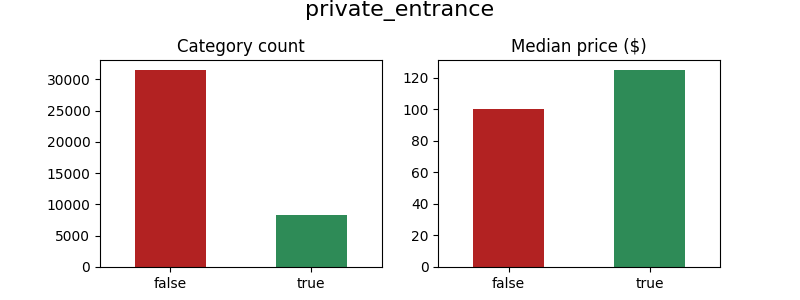
\includegraphics[width=\linewidth]{figures/amenities/group1/private_entrance.png}
    %\caption{Caption 1}
    \vspace{0.5cm}
    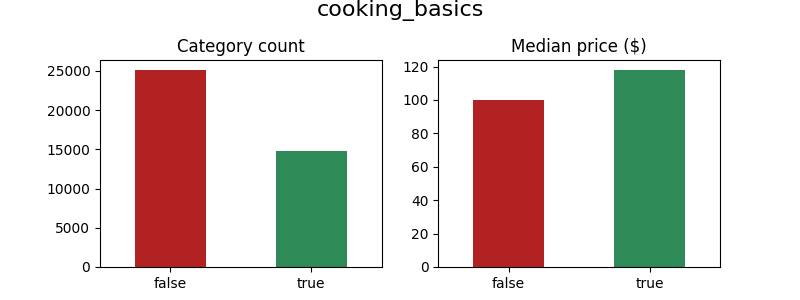
\includegraphics[width=\linewidth]{figures/amenities/group1/cooking_basics.png}
    %\caption{Caption 2}
    \label{fig:private-entrance-and-cooking-basics}
\end{figure}


% Amenity Group 2
\begin{figure}[H]
\centering
\caption{TV and Internet}
    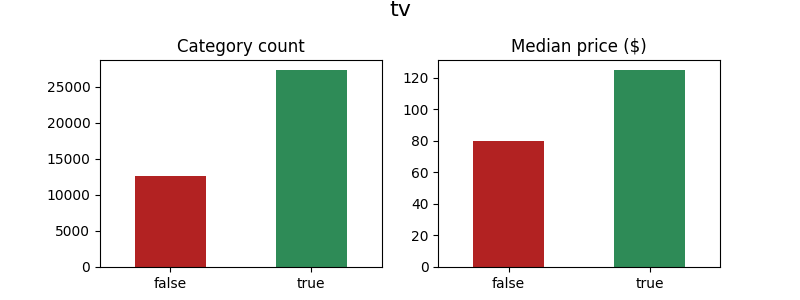
\includegraphics[width=\linewidth]{figures/amenities/group2/tv.png}
    %\caption{Caption 1}
    \vspace{0.5cm}
    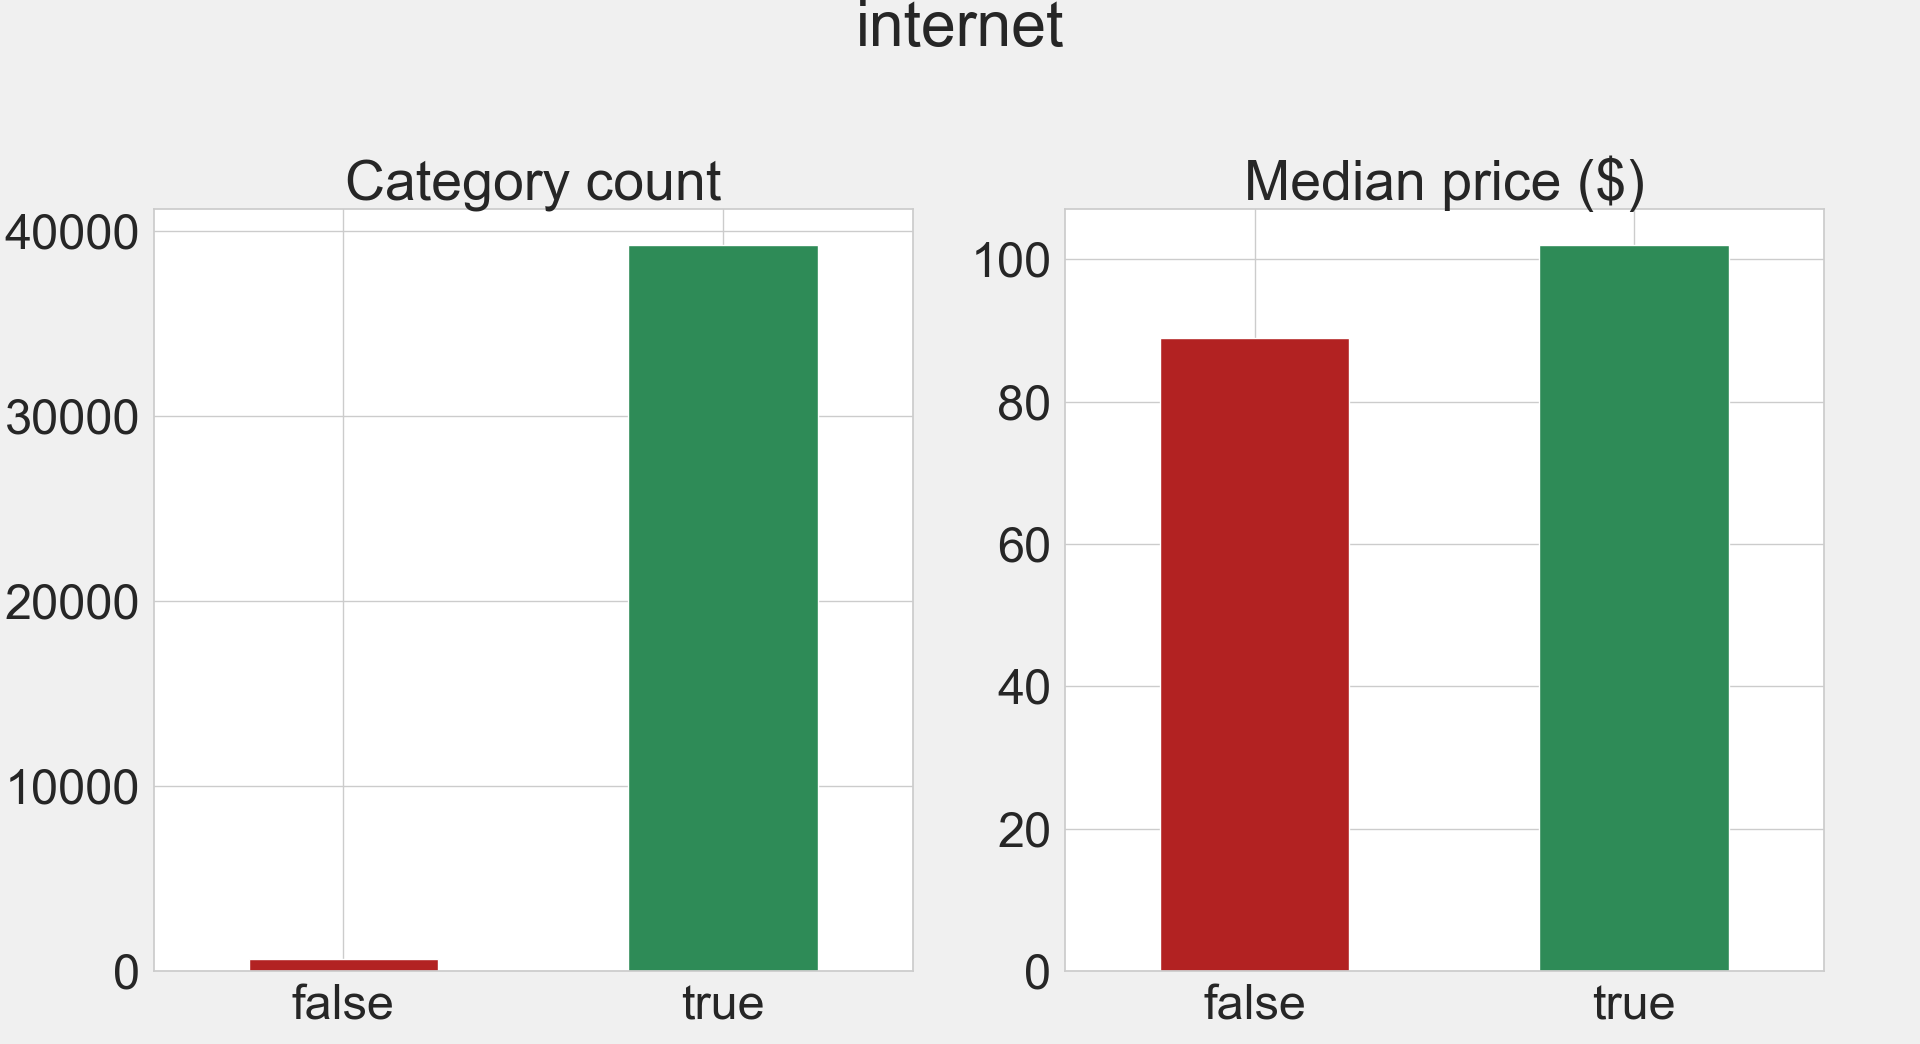
\includegraphics[width=\linewidth]{figures/amenities/group2/internet.png}
    %\caption{Caption 2}
    \label{fig:tv-and-internet}
\end{figure}

\begin{figure}[H]
\centering
    \caption{Air Conditioner}
    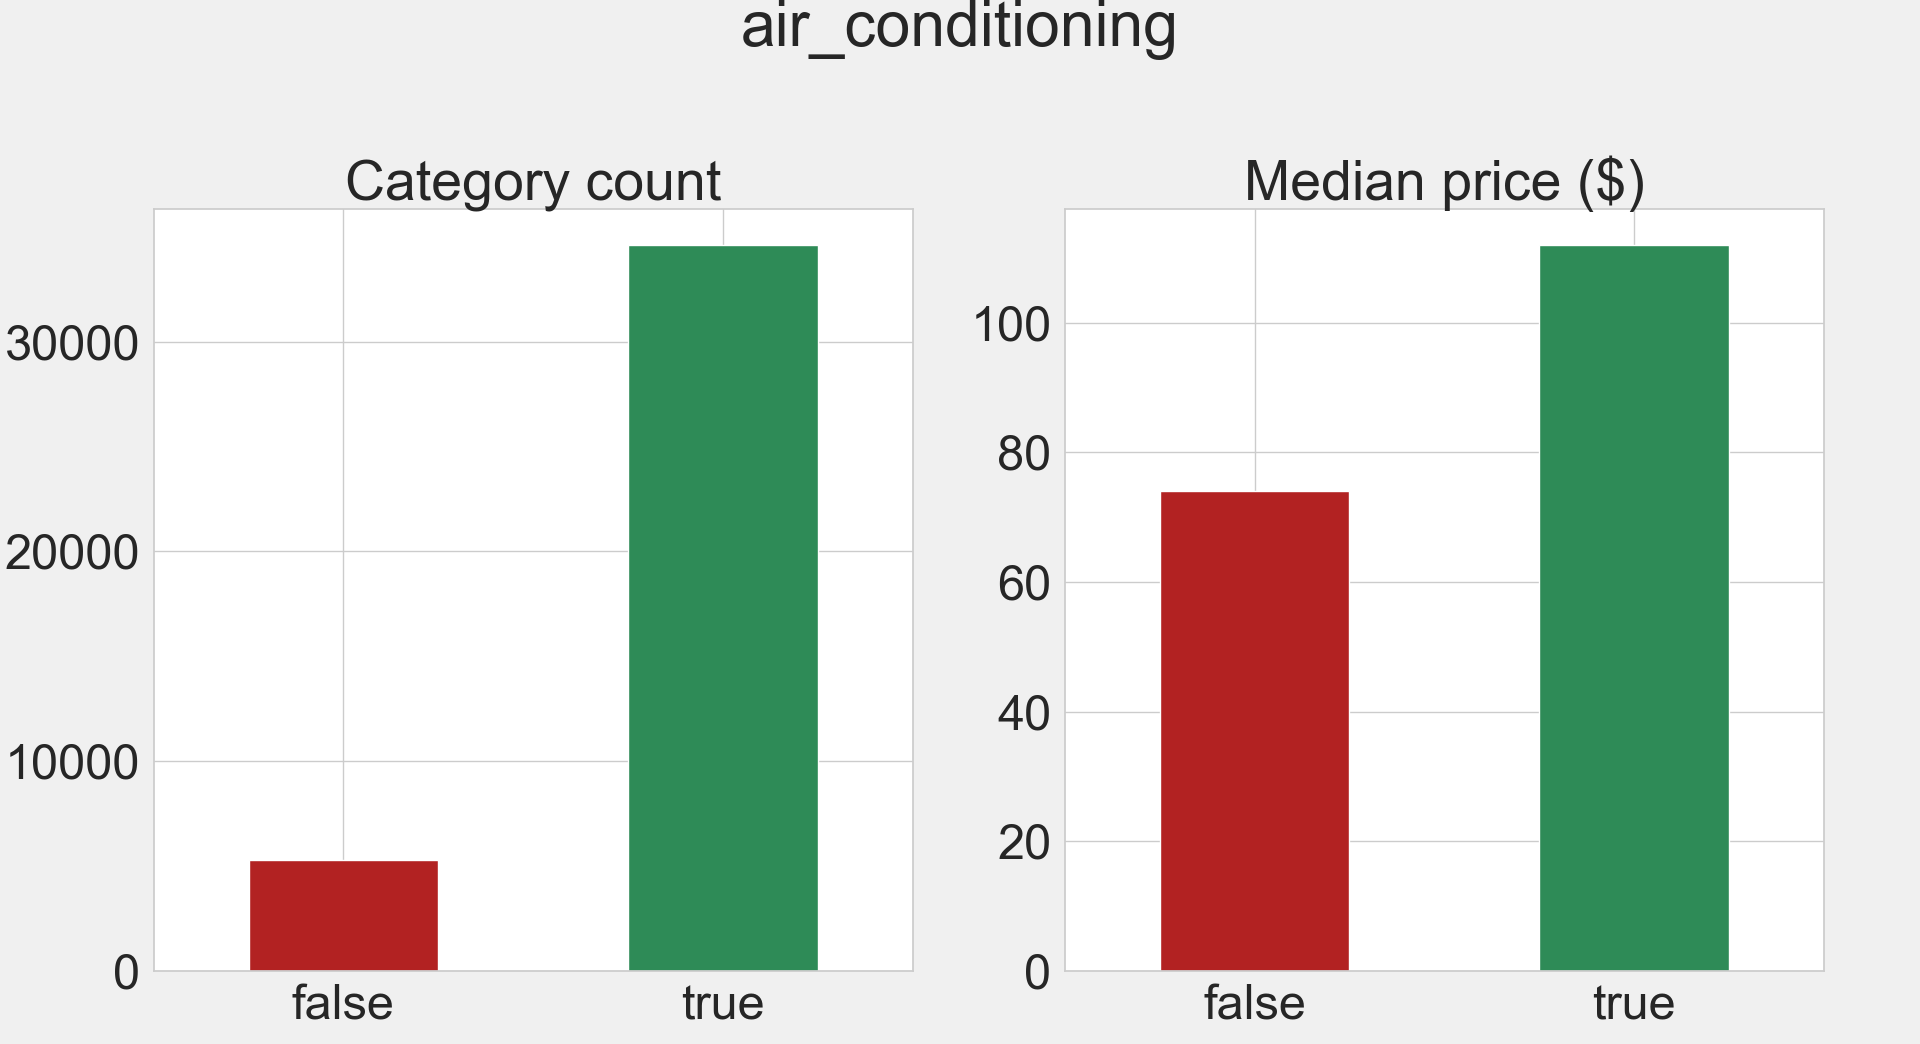
\includegraphics[width=\linewidth]{figures/amenities/group2/air_conditioning.png}
    \label{fig:air-conditioner}
\end{figure}

% Amenity Group 3
\begin{figure}[H]
\centering
    \caption{Parking and Host Greeting}
    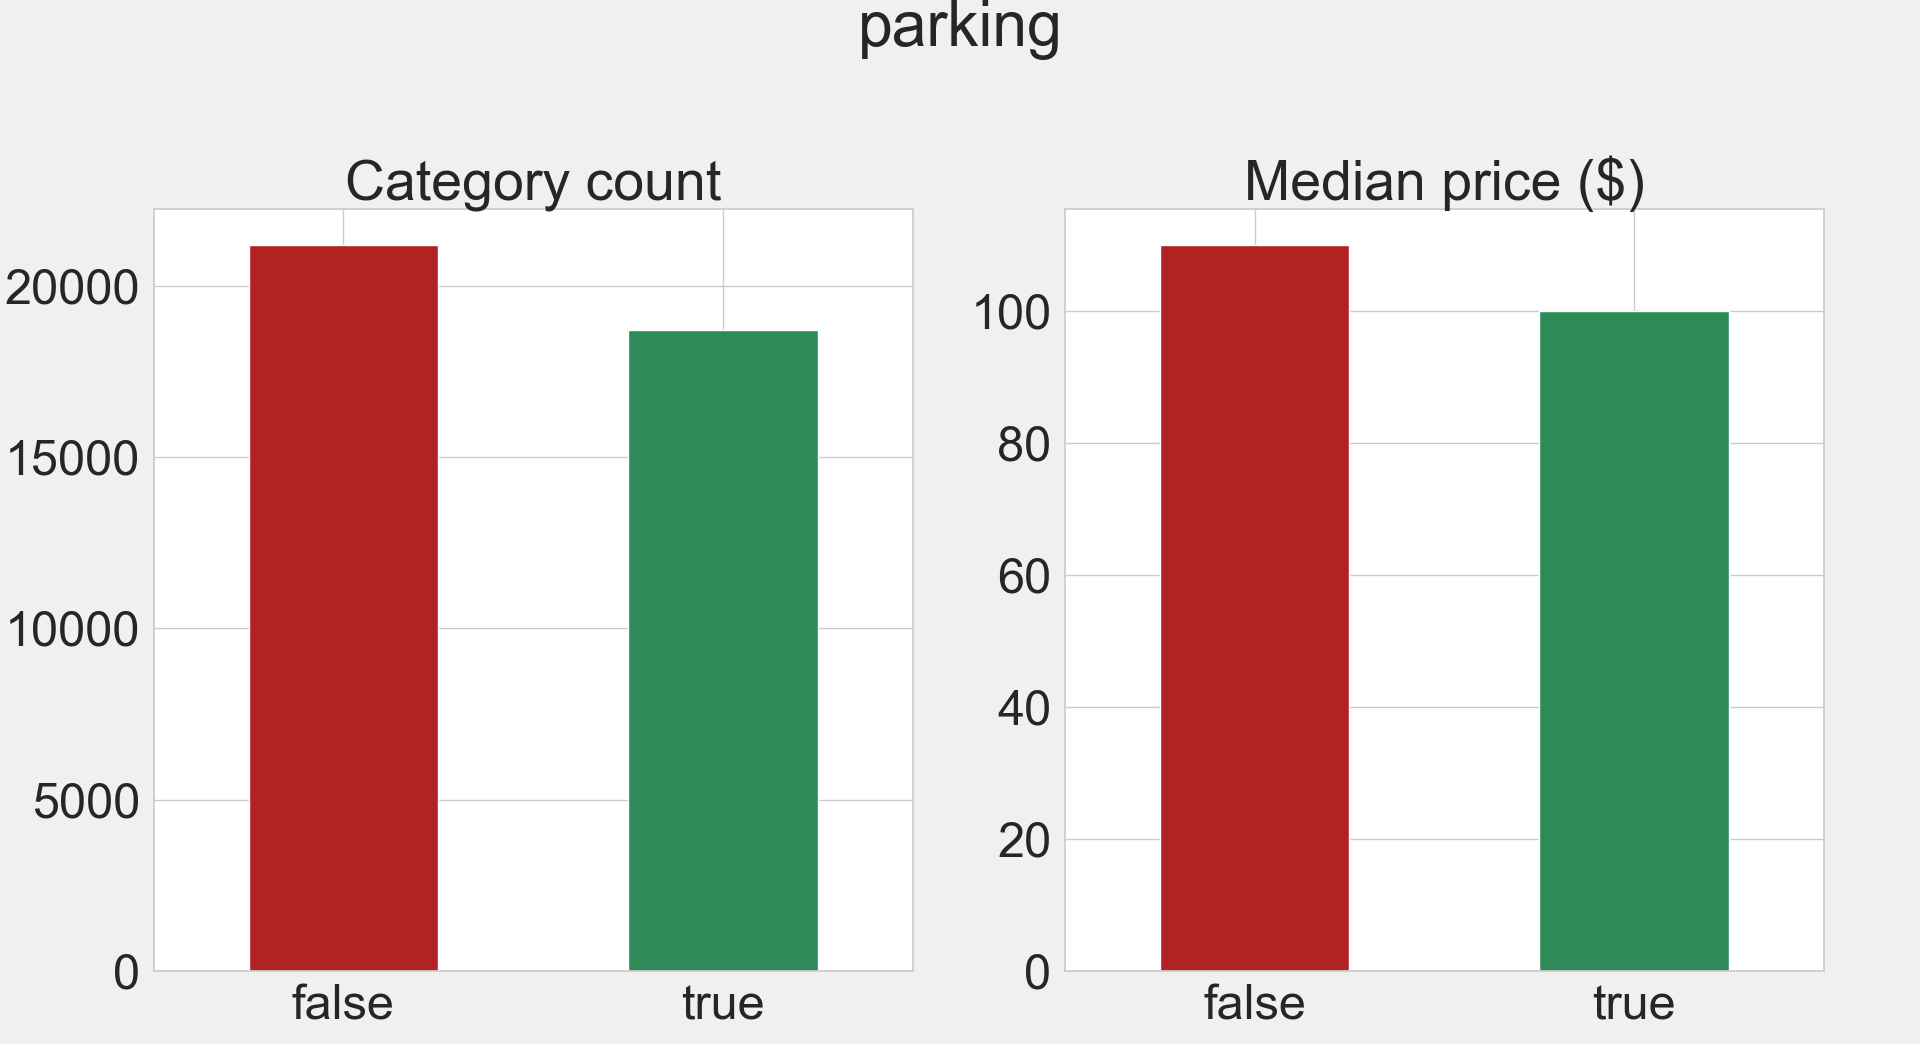
\includegraphics[width=\linewidth]{figures/amenities/group3/parking.png}
    \vspace{0.5cm}
    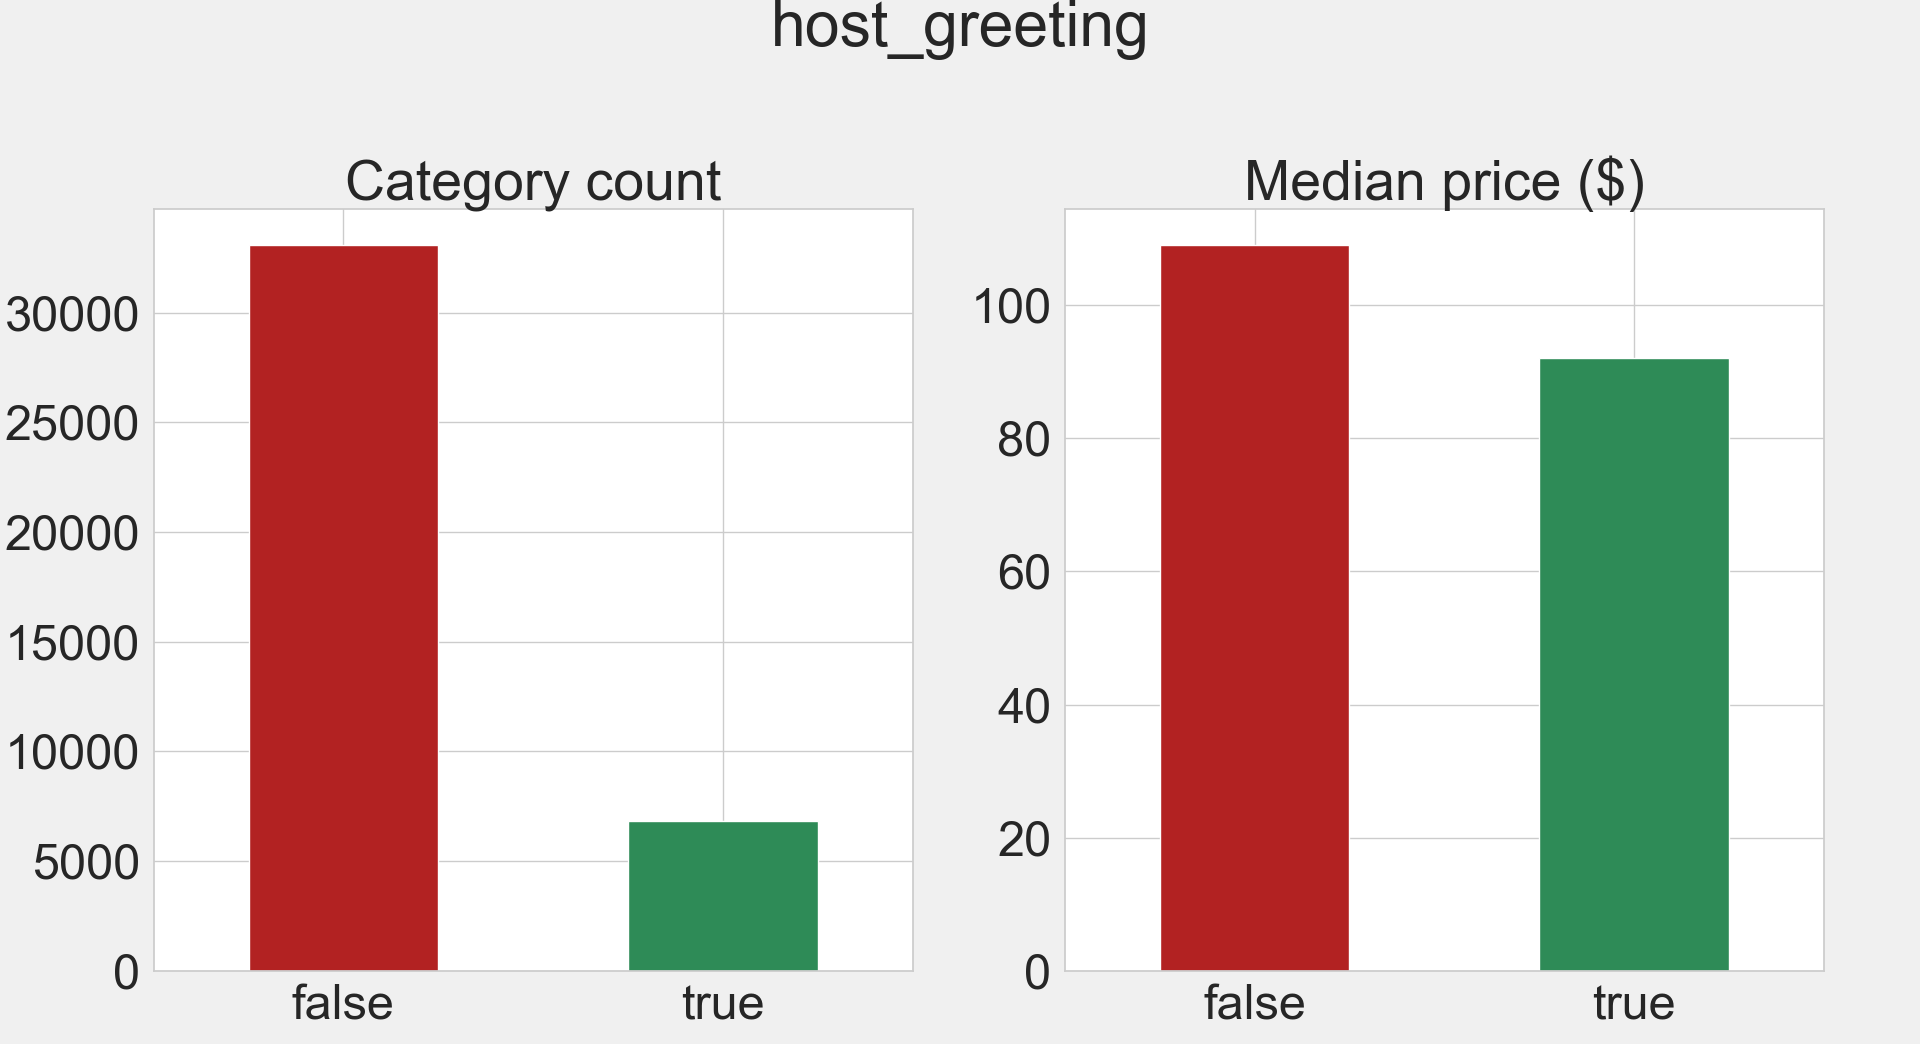
\includegraphics[width=\linewidth]{figures/amenities/group3/host_greetings.png}
    \label{fig:parking-and-host-greeting}
\end{figure}


\begin{figure}[H] \centering
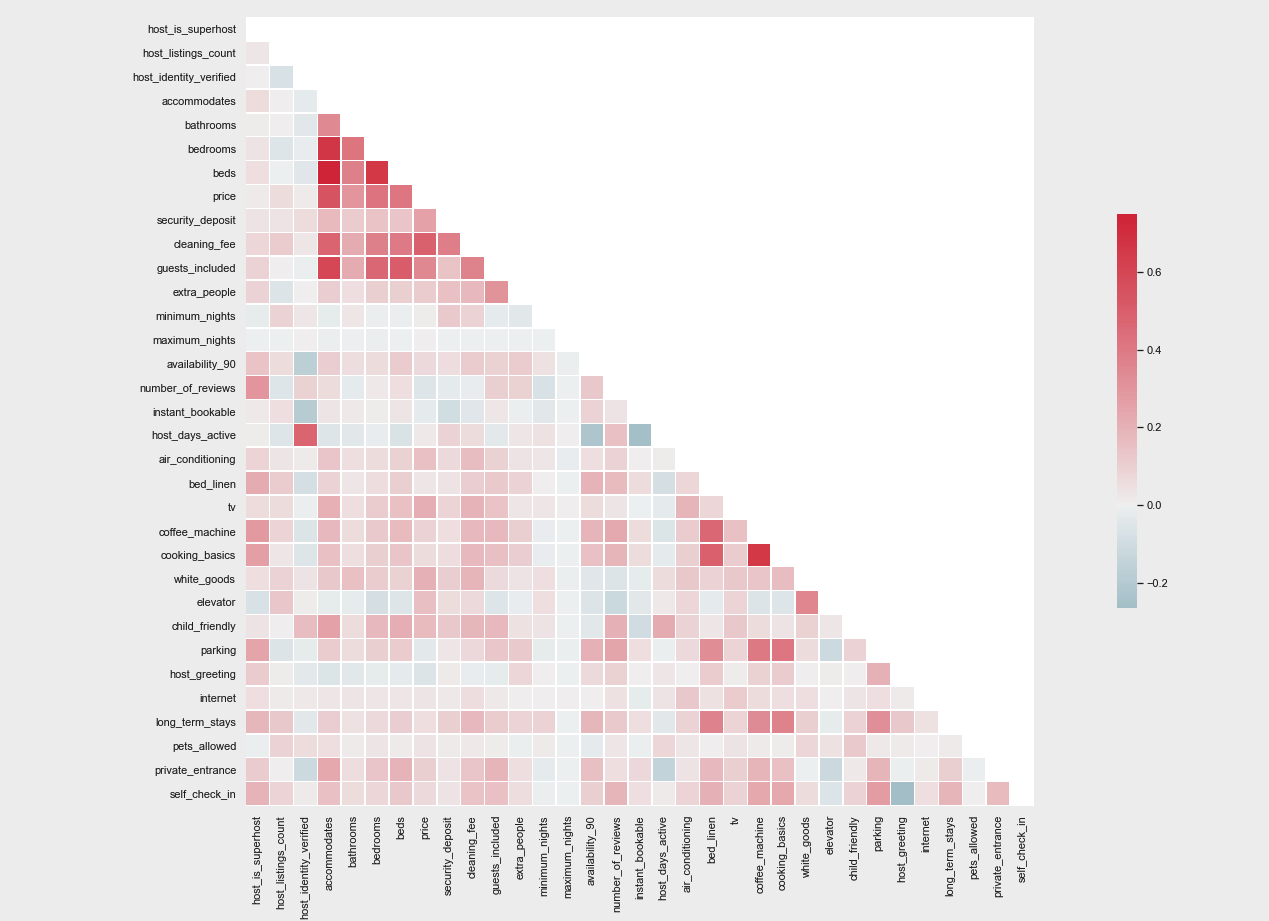
\includegraphics[width=\textwidth,keepaspectratio]{correlation-matrix.png}
\caption{Correlation Matrix}
\label{fig:correlation-matrix}
\end{figure}

\begin{figure}[H] \centering
\caption{Histogram of Feature Distribution}
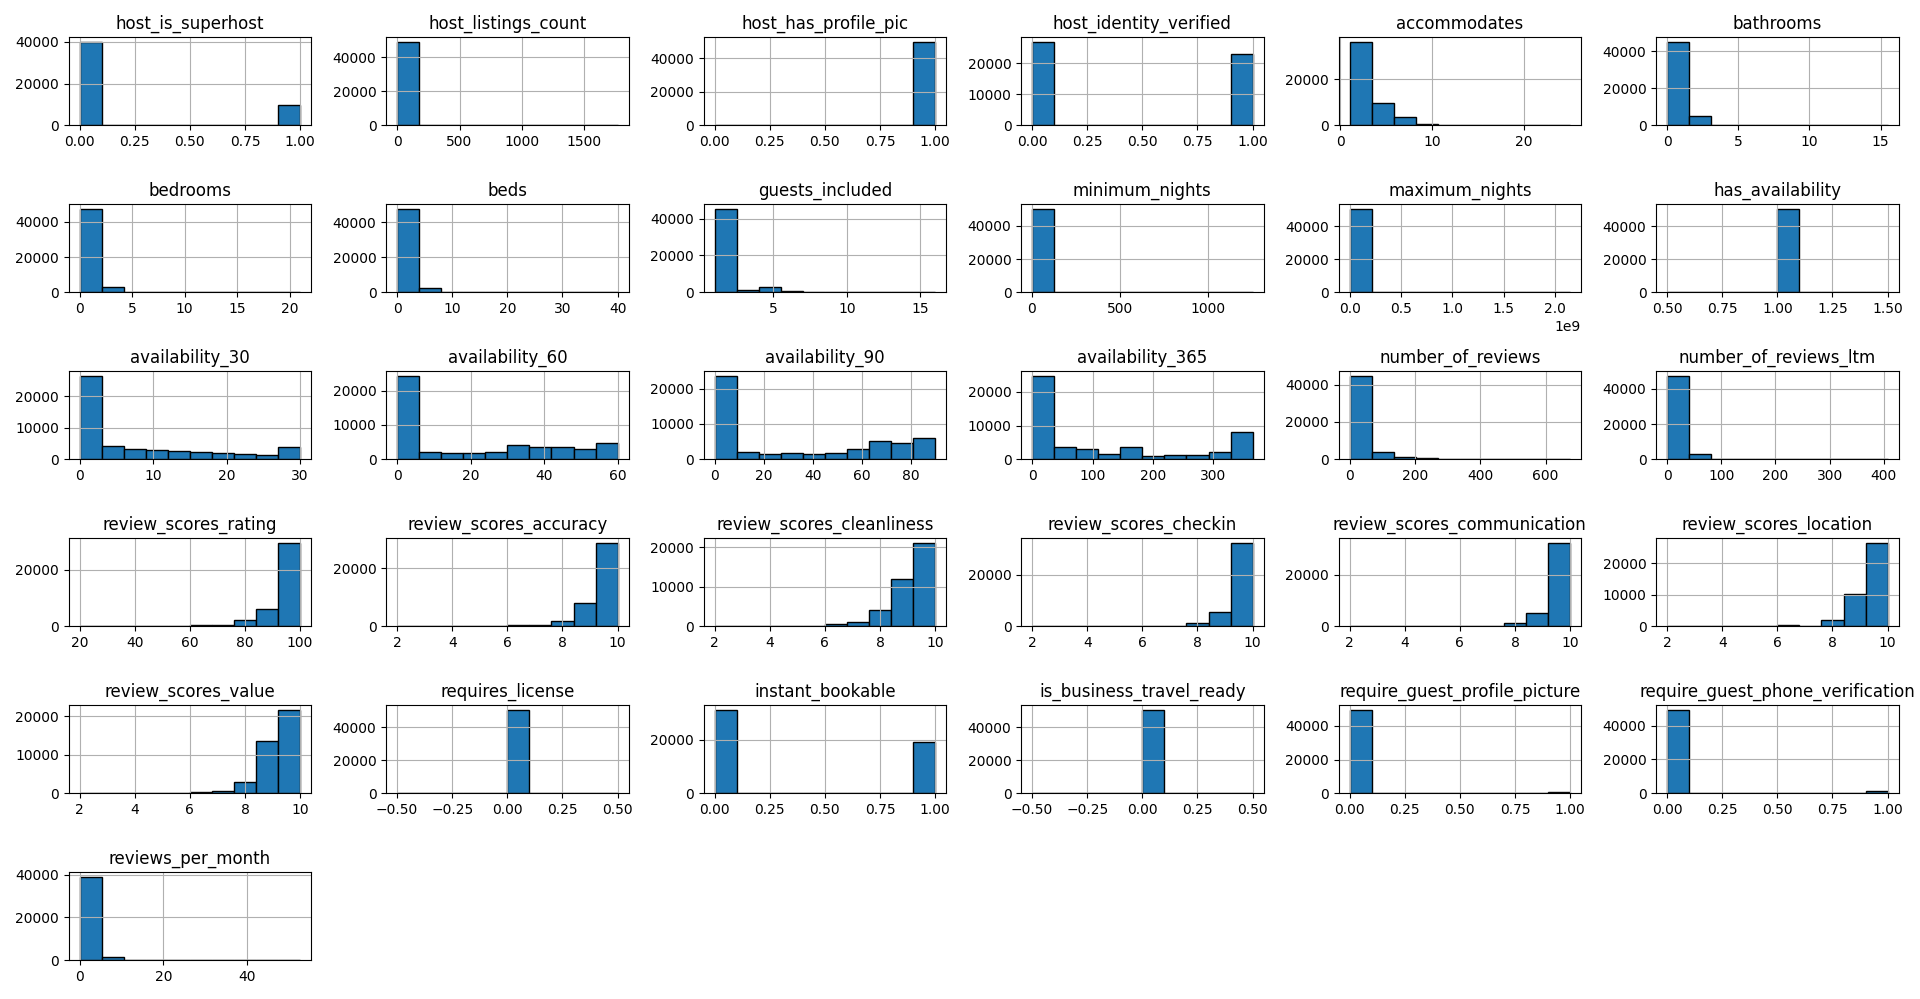
\includegraphics[width=\textwidth]{Figure_0_histogram.png}
\label{fig:histogram-feature-distribution}
\end{figure}

% from pre_processing.py
%Other than availability_90 and host_days_active, the remaining numerical
%features are all postively skewed and could benefit from log transformation.
\begin{figure}[H] \centering
\caption{Histogram of Numerical Feature Distribution Before Log Transform }
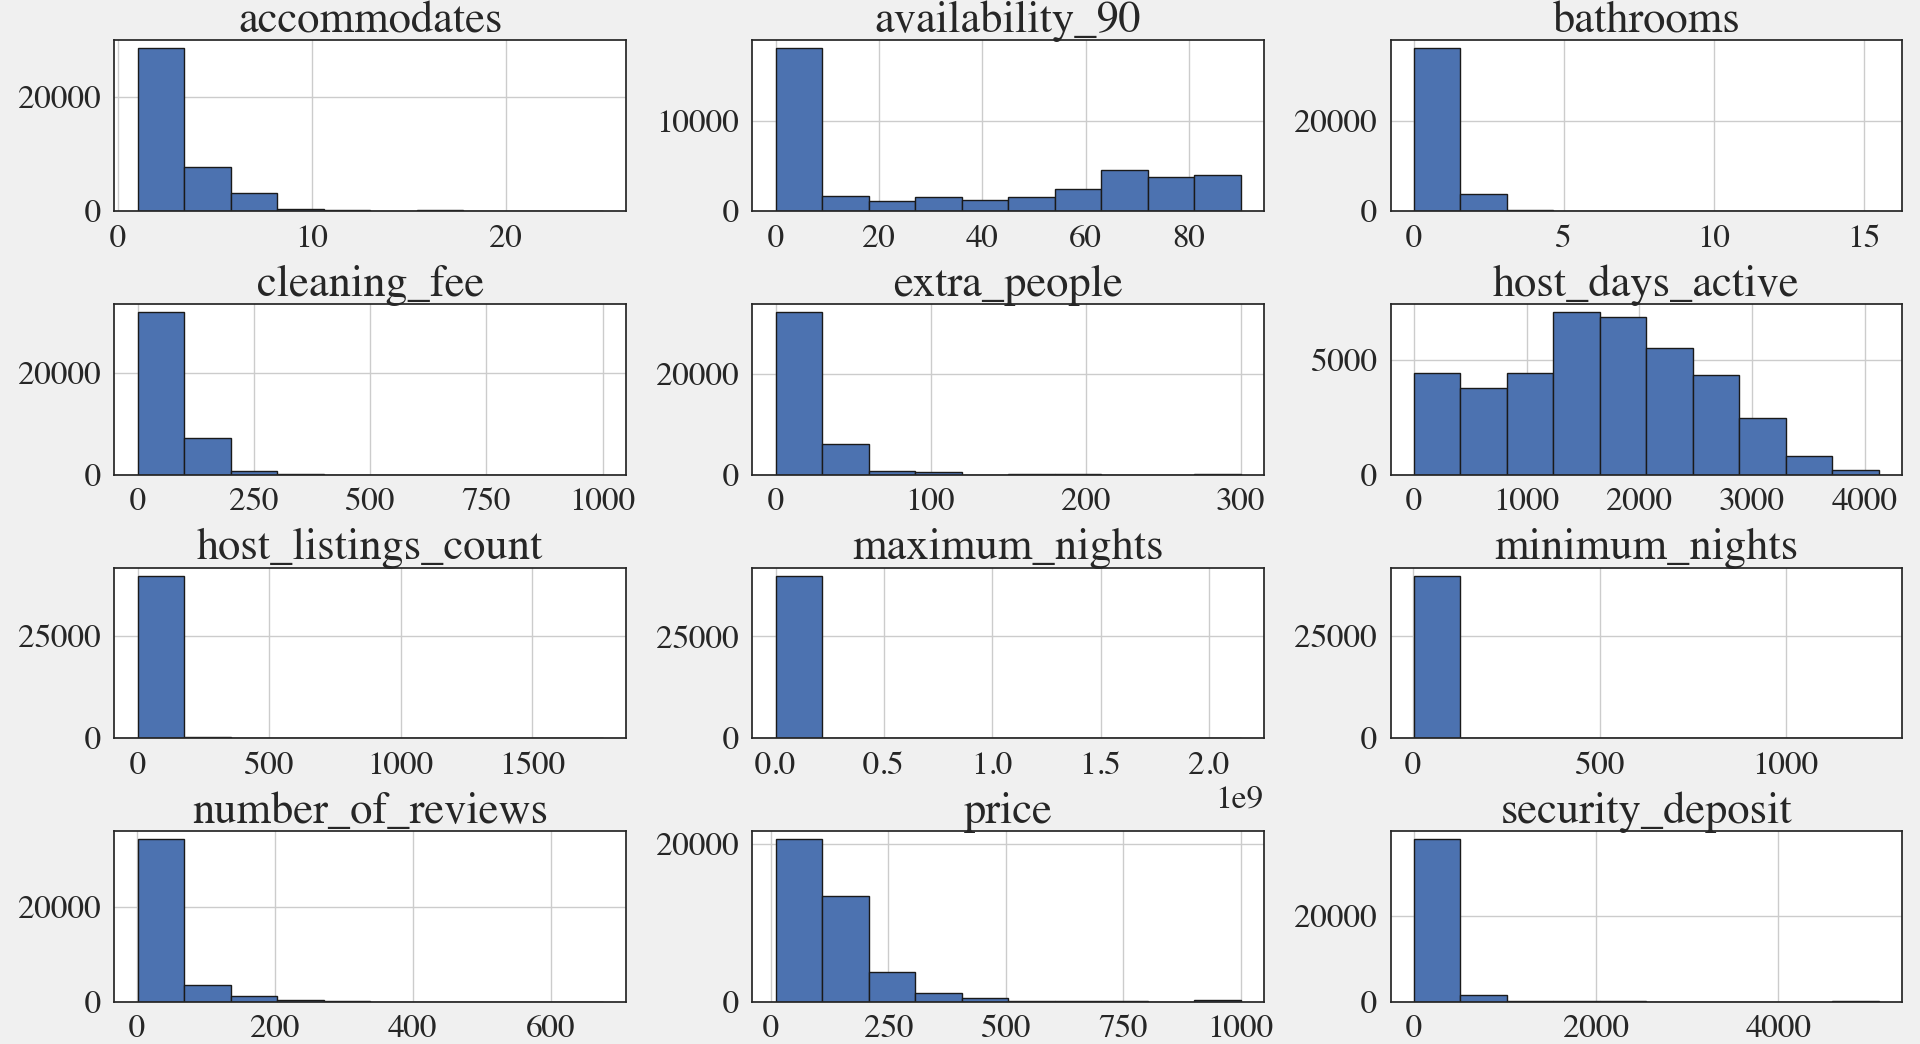
\includegraphics[width=\textwidth]{before-log.png}
\label{fig:histogram-before-transform}
\end{figure}

% from pre_processing.py
\begin{figure}[H] \centering
\caption{Histogram of Numerical Feature Distribution After Log Transform }
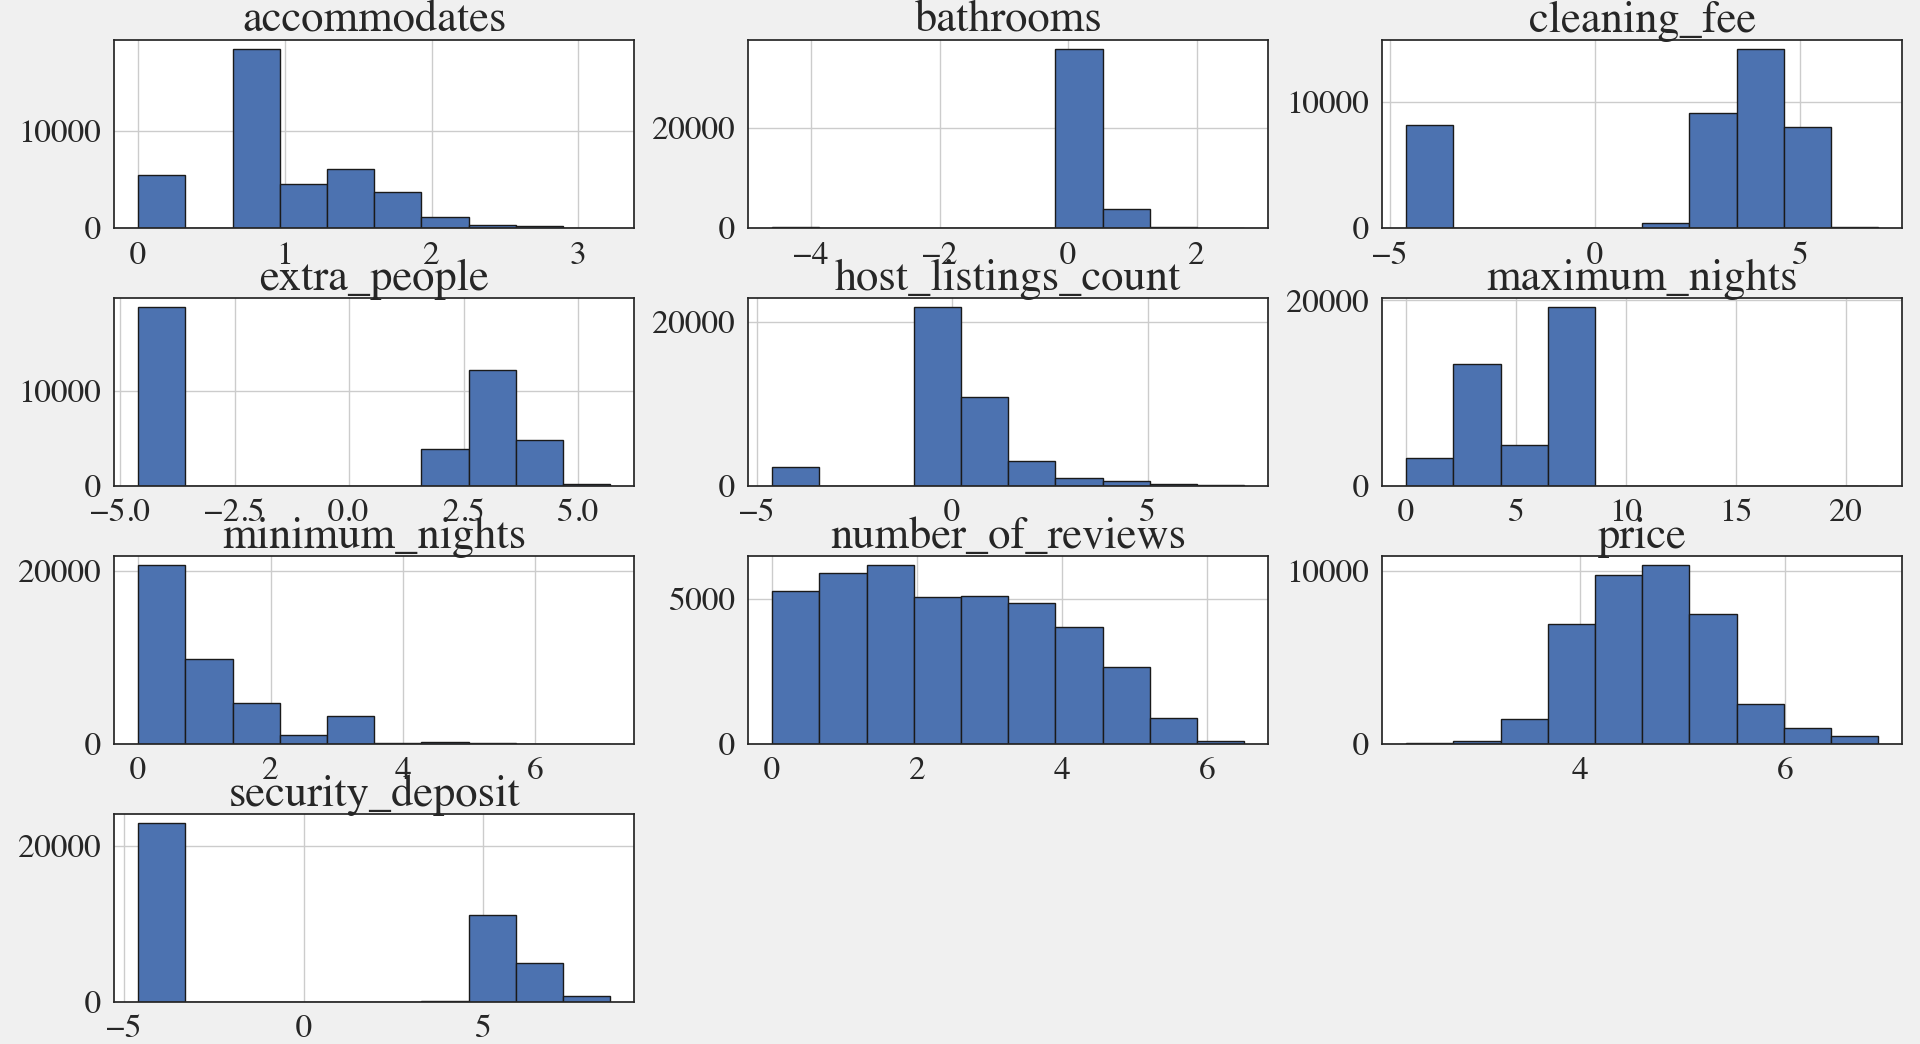
\includegraphics[width=\textwidth]{after-log.png}
\label{fig:histogram-after-transform}
\end{figure}
